Dưới đây là phân tích chi tiết các use case của hệ thống Social Commerce, được phân loại theo từng module chính. Mỗi module bao gồm danh sách use case và đặc tả chi tiết cho từng use case, bao gồm tên, tác nhân, mô tả, kích hoạt, điều kiện tiên quyết, điều kiện sau, luồng sự kiện chính, luồng thay thế, ngoại lệ và ghi chú.

\subsection{Use Case toàn hệ thống}

\begin{figure}[H]
\centering
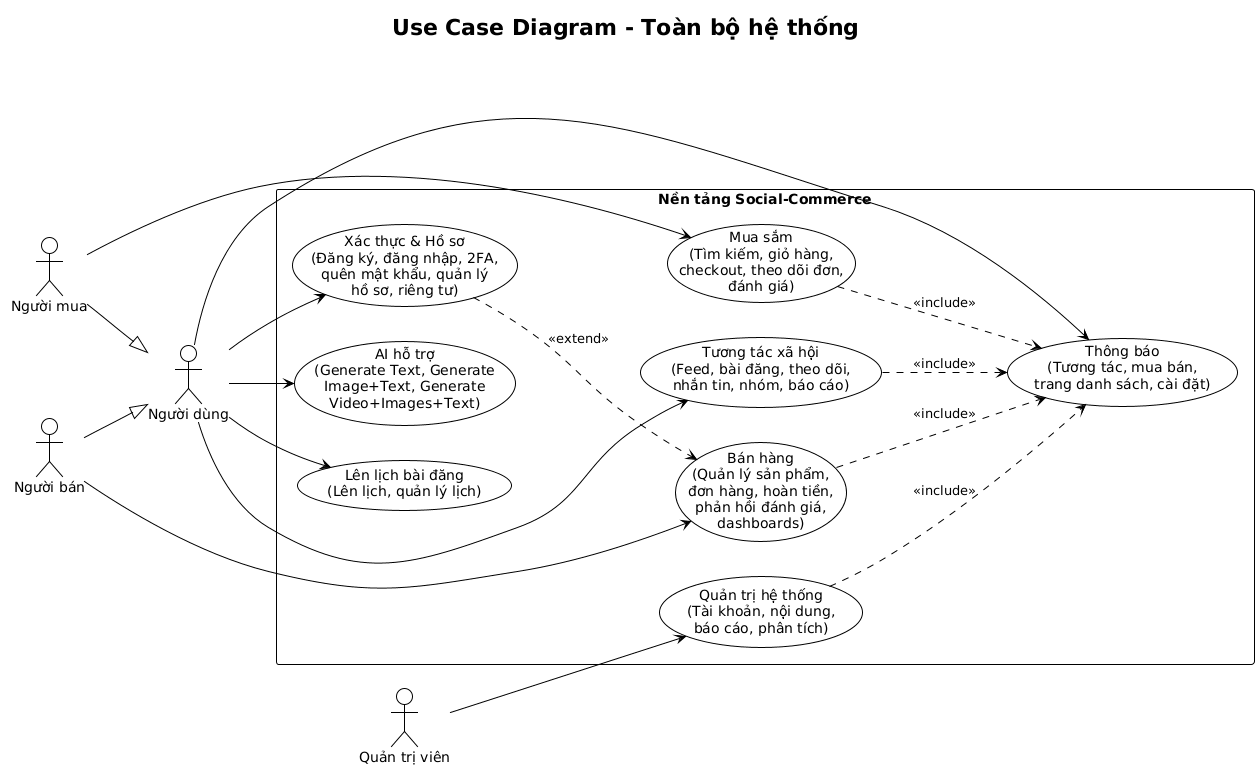
\includegraphics[width=\textwidth]{Images/Usecases/UC-All-System.png}
\caption{Sơ đồ Use Case tổng quan cho toàn hệ thống Social Commerce}
\label{fig:usecase-total}
\end{figure}

\subsection{Module 1: Quản lý Người dùng và Xác thực}
\subsubsection{Module 1: Quản lý Người dùng và Xác thực}
Module này bao gồm các chức năng cốt lõi liên quan đến việc tạo lập, xác thực và quản lý tài khoản người dùng trong hệ thống.

\begin{figure}[H]
\centering
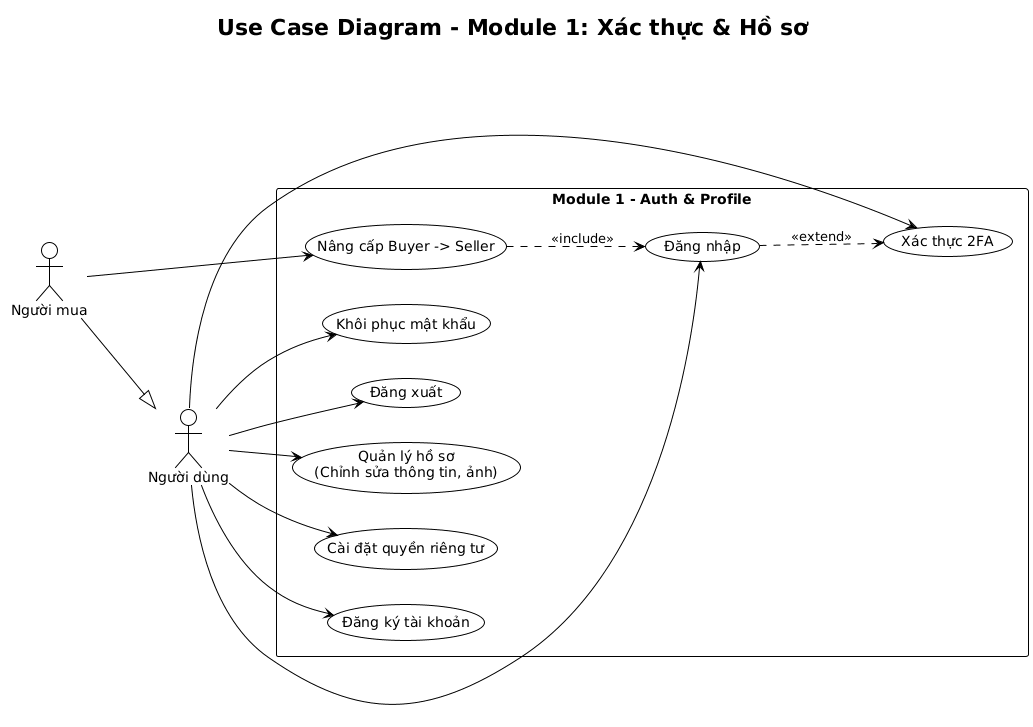
\includegraphics[width=\textwidth]{Images/Usecases/UC-M1-Auth.png}
\caption{Sơ đồ Use Case cho Module 1: Quản lý Người dùng và Xác thực}
\label{fig:usecase-module1}
\end{figure}

% Cấu hình giãn dòng cho bảng dễ đọc hơn
\renewcommand{\arraystretch}{1.3}

% =====================================================
% UC1.1: ĐĂNG KÝ TÀI KHOẢN
% =====================================================
\begin{table}[H]
\centering
\begin{tabularx}{\textwidth}{|l|X|}
\hline
\textbf{Tên Use Case} & \textbf{UC1.1: Đăng ký tài khoản} \\ \hline
\textbf{Tác nhân} & Người dùng chưa đăng nhập \\ \hline
\textbf{Mô tả} & Cho phép người dùng mới tạo một tài khoản trên hệ thống Social Commerce với vai trò mặc định là ``Người mua'' (Buyer). \\ \hline
\textbf{Kích hoạt} & Người dùng nhấn vào nút ``Đăng ký'' trên giao diện. \\ \hline
\textbf{Điều kiện tiên quyết} & 
\begin{itemize}
    \item Người dùng chưa đăng nhập vào hệ thống.
    \item Người dùng có một địa chỉ email hợp lệ và chưa được sử dụng để đăng ký.
\end{itemize} \\ \hline
\textbf{Điều kiện sau} & 
\begin{itemize}
    \item Tài khoản mới được tạo với trạng thái ``chưa xác thực''.
    \item Vai trò người dùng được gán là Buyer.
    \item Hệ thống gửi email/tin nhắn xác thực tài khoản.
    \item Người dùng được chuyển hướng đến trang yêu cầu xác thực.
\end{itemize} \\ \hline
\textbf{Luồng sự kiện chính} & 
\begin{enumerate}
    \item Người dùng truy cập trang Đăng ký.
    \item Người dùng nhập các thông tin bắt buộc.
    \item Người dùng nhấn nút ``Đăng ký''.
    \item Hệ thống kiểm tra tính hợp lệ của dữ liệu.
    \item Hệ thống kiểm tra email đã tồn tại hay chưa.
    \item Hệ thống tạo người dùng mới với trạng thái ``chưa xác thực''.
    \item Hệ thống gửi email/SMS xác thực.
    \item Hệ thống hiển thị thông báo thành công và yêu cầu xác thực.
\end{enumerate} \\ \hline
\textbf{Ngoại lệ} & 
\begin{itemize}
    \item E1: Email không hợp lệ $\rightarrow$ Báo lỗi ``Định dạng email không hợp lệ''.
    \item E2: Mật khẩu xác nhận không khớp $\rightarrow$ Báo lỗi ``Mật khẩu xác nhận không khớp''.
    \item E3: Email đã tồn tại $\rightarrow$ Báo lỗi ``Email này đã được sử dụng''.
    \item E4: Lỗi gửi email $\rightarrow$ Báo lỗi và đề nghị thử lại.
\end{itemize} \\ \hline
\textbf{Ghi chú} & Đây là bước đầu tiên để tham gia vào hệ sinh thái Social Commerce. \\ \hline
\end{tabularx}
\caption{Đặc tả Use Case Đăng ký tài khoản}
\end{table}

% =====================================================
% UC1.2: ĐĂNG NHẬP
% =====================================================
\begin{table}[H]
\centering
\begin{tabularx}{\textwidth}{|l|X|}
\hline
\textbf{Tên Use Case} & \textbf{UC1.2: Đăng nhập vào hệ thống} \\ \hline
\textbf{Tác nhân} & Người dùng chưa đăng nhập \\ \hline
\textbf{Mô tả} & Cho phép người dùng đã có tài khoản truy cập vào hệ thống bằng email và mật khẩu. \\ \hline
\textbf{Kích hoạt} & Người dùng nhấn vào nút ``Đăng nhập'' sau khi điền thông tin. \\ \hline
\textbf{Điều kiện tiên quyết} & Người dùng có một tài khoản đã đăng ký và xác thực. \\ \hline
\textbf{Điều kiện sau} & 
\begin{itemize}
    \item Hệ thống tạo một phiên làm việc (session) cho người dùng.
    \item Hệ thống cấp một JSON Web Token (JWT) để xác thực.
    \item Người dùng được chuyển hướng đến trang chủ.
\end{itemize} \\ \hline
\textbf{Luồng sự kiện chính} & 
\begin{enumerate}
    \item Người dùng truy cập trang Đăng nhập.
    \item Người dùng nhập email và mật khẩu.
    \item Người dùng nhấn nút ``Đăng nhập''.
    \item Hệ thống xác thực thông tin.
    \item Nếu thông tin chính xác và tài khoản không bật 2FA, hệ thống tạo JWT và chuyển hướng người dùng.
\end{enumerate} \\ \hline
\textbf{Ngoại lệ} & 
\begin{itemize}
    \item E1: Sai email hoặc mật khẩu $\rightarrow$ Báo lỗi ``Thông tin đăng nhập không chính xác''.
    \item E2: Tài khoản chưa được xác thực $\rightarrow$ Báo lỗi và yêu cầu xác thực.
    \item E3: Tài khoản bị khóa $\rightarrow$ Báo lỗi ``Tài khoản của bạn đã bị khóa''.
\end{itemize} \\ \hline
\textbf{Ghi chú} & Quá trình xác thực sử dụng JWT để đảm bảo an toàn. \\ \hline
\end{tabularx}
\caption{Đặc tả Use Case Đăng nhập}
\end{table}

% =====================================================
% UC1.3: XÁC THỰC 2 YẾU TỐ (2FA)
% =====================================================
\begin{table}[H]
\centering
\begin{tabularx}{\textwidth}{|l|X|}
\hline
\textbf{Tên Use Case} & \textbf{UC1.3: Sử dụng xác thực hai yếu tố (2FA)} \\ \hline
\textbf{Tác nhân} & Người dùng \\ \hline
\textbf{Mô tả} & Cung cấp một lớp bảo mật bổ sung khi đăng nhập bằng mã xác thực tạm thời. \\ \hline
\textbf{Kích hoạt} & Người dùng có bật 2FA và vừa nhập đúng mật khẩu ở bước đăng nhập. \\ \hline
\textbf{Điều kiện tiên quyết} & 
\begin{itemize}
    \item Người dùng đã kích hoạt tính năng 2FA.
    \item Người dùng đã nhập chính xác email và mật khẩu.
\end{itemize} \\ \hline
\textbf{Điều kiện sau} & 
\begin{itemize}
    \item Danh tính người dùng được xác thực hoàn toàn.
    \item Người dùng được đăng nhập thành công.
\end{itemize} \\ \hline
\textbf{Luồng sự kiện chính} & 
\begin{enumerate}
    \item Hệ thống hiển thị trang nhập mã 2FA.
    \item Người dùng lấy mã từ email (hoặc ứng dụng Authenticator).
    \item Người dùng nhập mã 2FA.
    \item Người dùng nhấn ``Xác nhận''.
    \item Hệ thống kiểm tra mã.
    \item Nếu mã hợp lệ, quá trình đăng nhập hoàn tất.
\end{enumerate} \\ \hline
\textbf{Ngoại lệ} & 
\begin{itemize}
    \item E1: Nhập sai mã 2FA $\rightarrow$ Báo lỗi ``Mã xác thực không chính xác''.
    \item E2: Mã 2FA hết hạn $\rightarrow$ Báo lỗi và yêu cầu thử lại.
\end{itemize} \\ \hline
\textbf{Ghi chú} & Tính năng này tùy chọn và quan trọng cho tài khoản người bán. \\ \hline
\end{tabularx}
\caption{Đặc tả Use Case Xác thực 2FA}
\end{table}

% =====================================================
% UC1.4: KHÔI PHỤC MẬT KHẨU
% =====================================================
\begin{table}[H]
\centering
\begin{tabularx}{\textwidth}{|l|X|}
\hline
\textbf{Tên Use Case} & \textbf{UC1.4: Khôi phục mật khẩu} \\ \hline
\textbf{Tác nhân} & Người dùng chưa đăng nhập \\ \hline
\textbf{Mô tả} & Cho phép người dùng đặt lại mật khẩu trong trường hợp họ quên. \\ \hline
\textbf{Kích hoạt} & Người dùng nhấn vào liên kết ``Quên mật khẩu?'' trên trang Đăng nhập. \\ \hline
\textbf{Điều kiện tiên quyết} & 
\begin{itemize}
    \item Người dùng có một tài khoản đã đăng ký.
    \item Người dùng có quyền truy cập vào email đã đăng ký.
\end{itemize} \\ \hline
\textbf{Điều kiện sau} & Mật khẩu của người dùng được cập nhật thành công. \\ \hline
\textbf{Luồng sự kiện chính} & 
\begin{enumerate}
    \item Người dùng nhấn ``Quên mật khẩu?''.
    \item Hệ thống yêu cầu người dùng nhập email.
    \item Người dùng nhập email và nhấn ``Gửi''.
    \item Hệ thống gửi email chứa liên kết hoặc mã OTP.
    \item Người dùng làm theo hướng dẫn trong email.
    \item Hệ thống chuyển hướng đến trang tạo mật khẩu mới.
    \item Người dùng nhập mật khẩu mới và xác nhận.
    \item Người dùng nhấn ``Lưu thay đổi''.
    \item Hệ thống cập nhật mật khẩu và thông báo thành công.
\end{enumerate} \\ \hline
\textbf{Ngoại lệ} & 
\begin{itemize}
    \item E1: Email không tồn tại $\rightarrow$ Hệ thống hiển thị thông báo chung để bảo mật (tránh lộ danh tính user).
    \item E2: Liên kết/mã OTP hết hạn hoặc không hợp lệ $\rightarrow$ Báo lỗi và yêu cầu làm lại.
    \item E3: Mật khẩu mới không khớp $\rightarrow$ Báo lỗi.
\end{itemize} \\ \hline
\end{tabularx}
\caption{Đặc tả Use Case Khôi phục mật khẩu}
\end{table}

% =====================================================
% UC1.5: ĐĂNG XUẤT
% =====================================================
\begin{table}[H]
\centering
\begin{tabularx}{\textwidth}{|l|X|}
\hline
\textbf{Tên Use Case} & \textbf{UC1.5: Đăng xuất} \\ \hline
\textbf{Tác nhân} & Người dùng \\ \hline
\textbf{Mô tả} & Cho phép người dùng kết thúc phiên làm việc hiện tại một cách an toàn. \\ \hline
\textbf{Kích hoạt} & Người dùng nhấn vào nút ``Đăng xuất''. \\ \hline
\textbf{Điều kiện tiên quyết} & Người dùng đang đăng nhập vào hệ thống. \\ \hline
\textbf{Điều kiện sau} & 
\begin{itemize}
    \item Phiên làm việc của người dùng bị hủy.
    \item JWT trên client bị xóa.
    \item Người dùng được chuyển hướng về trang chủ.
\end{itemize} \\ \hline
\textbf{Luồng sự kiện chính} & 
\begin{enumerate}
    \item Người dùng nhấn nút ``Đăng xuất''.
    \item Hệ thống hủy phiên làm việc và xóa token lưu trữ ở client.
    \item Hệ thống chuyển hướng người dùng về trang chủ.
\end{enumerate} \\ \hline
\end{tabularx}
\caption{Đặc tả Use Case Đăng xuất}
\end{table}

% =====================================================
% UC1.6: QUẢN LÝ HỒ SƠ CÁ NHÂN
% =====================================================
\begin{table}[H]
\centering
\begin{tabularx}{\textwidth}{|l|X|}
\hline
\textbf{Tên Use Case} & \textbf{UC1.6: Quản lý hồ sơ cá nhân} \\ \hline
\textbf{Tác nhân} & Người dùng \\ \hline
\textbf{Mô tả} & Cho phép người dùng xem và chỉnh sửa thông tin cá nhân, ảnh đại diện và ảnh bìa. \\ \hline
\textbf{Kích hoạt} & Người dùng truy cập trang cá nhân và chọn chức năng chỉnh sửa. \\ \hline
\textbf{Điều kiện tiên quyết} & Người dùng đang đăng nhập vào hệ thống. \\ \hline
\textbf{Điều kiện sau} & 
\begin{itemize}
    \item Thông tin cá nhân của người dùng được cập nhật.
    \item Thay đổi được hiển thị ngay lập tức.
\end{itemize} \\ \hline
\textbf{Luồng sự kiện chính} & 
\begin{enumerate}
    \item Người dùng vào trang hồ sơ cá nhân.
    \item Người dùng nhấn ``Chỉnh sửa hồ sơ''.
    \item Người dùng thay đổi thông tin.
    \item Người dùng nhấn ``Lưu thay đổi''.
    \item Hệ thống xác thực và cập nhật dữ liệu.
    \item Hệ thống hiển thị thông báo thành công.
\end{enumerate} \\ \hline
\textbf{Luồng thay thế} & A1: Người dùng nhấn ``Hủy'' $\rightarrow$ Các thay đổi sẽ không được lưu. \\ \hline
\textbf{Ngoại lệ} & 
\begin{itemize}
    \item E1: Lỗi tải lên hình ảnh $\rightarrow$ Báo lỗi tương ứng.
    \item E2: Dữ liệu nhập không hợp lệ $\rightarrow$ Báo lỗi tại trường dữ liệu đó.
\end{itemize} \\ \hline
\textbf{Ghi chú} & Giao diện quản lý cần trực quan và dễ sử dụng. \\ \hline
\end{tabularx}
\caption{Đặc tả Use Case Quản lý hồ sơ}
\end{table}

% =====================================================
% UC1.7: CÀI ĐẶT QUYỀN RIÊNG TƯ
% =====================================================
\begin{table}[H]
\centering
\begin{tabularx}{\textwidth}{|l|X|}
\hline
\textbf{Tên Use Case} & \textbf{UC1.7: Cài đặt quyền riêng tư cho tài khoản} \\ \hline
\textbf{Tác nhân} & Người dùng \\ \hline
\textbf{Mô tả} & Cho phép người dùng tùy chỉnh ai có thể xem hồ sơ, bài đăng hoặc danh sách người theo dõi. \\ \hline
\textbf{Kích hoạt} & Người dùng truy cập vào mục ``Cài đặt \& Quyền riêng tư''. \\ \hline
\textbf{Điều kiện tiên quyết} & Người dùng đang đăng nhập vào hệ thống. \\ \hline
\textbf{Điều kiện sau} & Các thiết lập quyền riêng tư của người dùng được cập nhật. \\ \hline
\textbf{Luồng sự kiện chính} & 
\begin{enumerate}
    \item Người dùng vào trang ``Cài đặt''.
    \item Người dùng chọn tab ``Quyền riêng tư''100.
    \item Người dùng thay đổi các tùy chọn.
    \item Người dùng nhấn ``Lưu thay đổi''.
    \item Hệ thống cập nhật và hiển thị thông báo thành công.
\end{enumerate} \\ \hline
\textbf{Ghi chú} & Tính năng này quan trọng để người dùng cảm thấy an toàn và kiểm soát thông tin. \\ \hline
\end{tabularx}
\caption{Đặc tả Use Case Cài đặt quyền riêng tư}
\end{table}

% =====================================================
% UC1.8: ĐĂNG KÝ NGƯỜI BÁN
% =====================================================
\begin{table}[H]
\centering
\begin{tabularx}{\textwidth}{|l|X|}
\hline
\textbf{Tên Use Case} & \textbf{UC1.8: Đăng ký trở thành Người bán} \\ \hline
\textbf{Tác nhân} & Người dùng (với vai trò Buyer) \\ \hline
\textbf{Mô tả} & Cung cấp quy trình để người dùng ``Người mua'' nâng cấp tài khoản thành ``Người bán''. \\ \hline
\textbf{Kích hoạt} & Người dùng nhấn vào nút ``Trở thành người bán''. \\ \hline
\textbf{Điều kiện tiên quyết} & 
\begin{itemize}
    \item Người dùng đang đăng nhập.
    \item Người dùng hiện có vai trò là Buyer.
\end{itemize} \\ \hline
\textbf{Điều kiện sau} & 
\begin{itemize}
    \item Hồ sơ đăng ký Seller được lưu và chuyển sang trạng thái chờ duyệt (\textit{REVIEWING}) sau khi hoàn thành các bước bắt buộc.
    \item Khi Admin phê duyệt, vai trò người dùng được cập nhật thành Seller.
\end{itemize} \\ \hline
\textbf{Luồng sự kiện chính} & 
\begin{enumerate}
    \item Người dùng truy cập trang ``Đăng ký Bán hàng'' và bắt đầu hồ sơ.
    \item Người dùng hoàn thành bước 1 (thông tin cá nhân/định danh).
    \item Người dùng hoàn thành bước 2 (thông tin kinh doanh).
    \item Người dùng hoàn thành bước 3 (thông tin ngân hàng) và nộp hồ sơ.
    \item Hệ thống chuyển hồ sơ sang trạng thái ``Đang xem xét''.
    \item Admin xét duyệt hồ sơ.
    \item Nếu được duyệt, hệ thống cập nhật vai trò thành Seller và gửi thông báo kết quả.
\end{enumerate} \\ \hline
\textbf{Luồng thay thế} & A1: Người dùng hủy bỏ quá trình đăng ký. \\ \hline
\textbf{Ngoại lệ} & 
\begin{itemize}
    \item E1: Thông tin ở bất kỳ bước nào không hợp lệ $\rightarrow$ Báo lỗi và yêu cầu sửa.
    \item E2: Hồ sơ bị từ chối $\rightarrow$ Hiển thị lý do từ chối để người dùng bổ sung.
\end{itemize} \\ \hline
\textbf{Ghi chú} & Đây là use case cốt lõi thể hiện mô hình ``buyer-to-seller'' của dự án. \\ \hline
\end{tabularx}
\caption{Đặc tả Use Case Đăng ký làm Người bán}
\end{table}

\subsection{Module 2: Tương tác Xã hội}
\subsubsection{Module 2: Tương tác Xã hội}
Module này tập trung vào các tính năng kết nối cộng đồng, chia sẻ nội dung và tương tác giữa người mua và người bán, tạo tiền đề cho các hoạt động thương mại.

\begin{figure}[H]
\centering
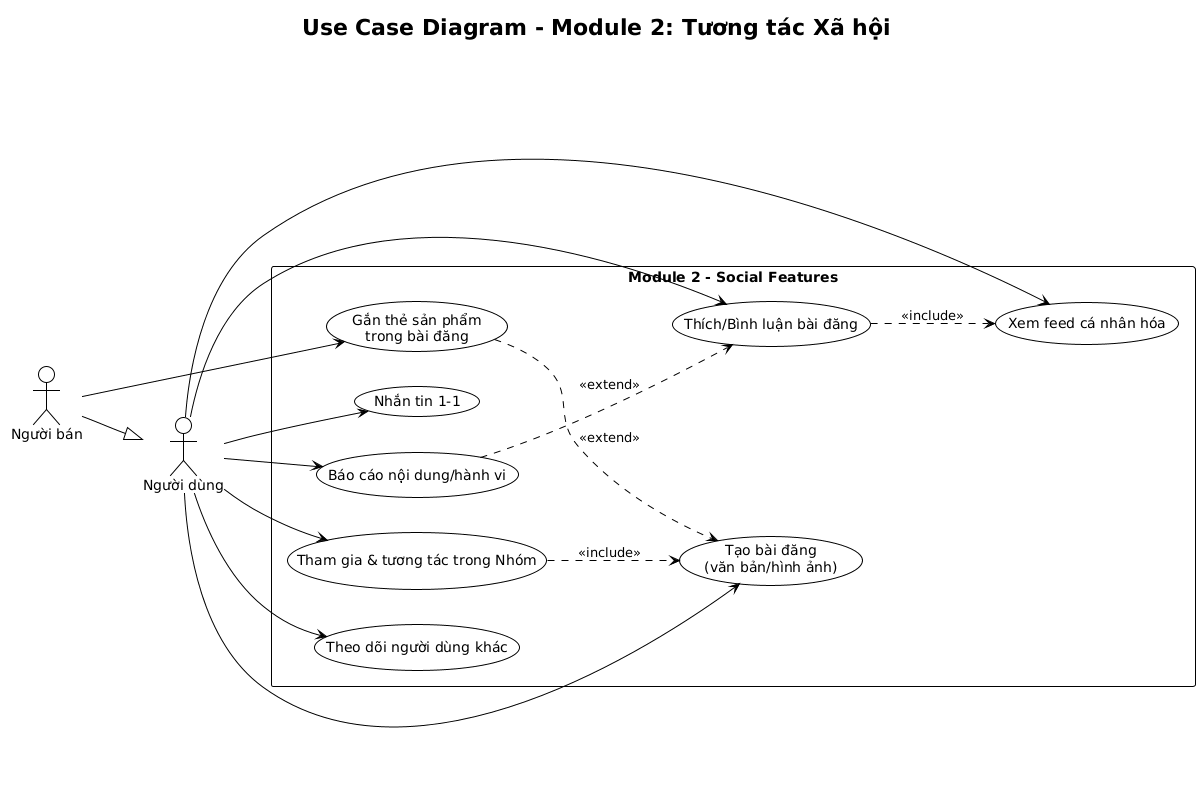
\includegraphics[width=\textwidth]{Images/Usecases/UC-M2-Social.png}
\caption{Sơ đồ Use Case cho Module 2: Tương tác Xã hội}
\label{fig:usecase-module2}
\end{figure}

% Cấu hình giãn dòng
\renewcommand{\arraystretch}{1.3}

% =====================================================
% UC2.1: XEM BẢNG TIN
% =====================================================
\begin{table}[H]
\centering
\begin{tabularx}{\textwidth}{|l|X|}
\hline
\textbf{Tên Use Case} & \textbf{UC2.1: Xem bảng tin (Feed) cá nhân hóa} \\ \hline
\textbf{Tác nhân} & Người dùng \\ \hline
\textbf{Mô tả} & Hiển thị một Bảng tin (Feed) được cá nhân hóa cho người dùng, ưu tiên hiển thị các bài đăng từ những người họ theo dõi và các bài viết có tương tác cao. \\ \hline
\textbf{Kích hoạt} & Người dùng truy cập vào trang chủ sau khi đăng nhập. \\ \hline
\textbf{Điều kiện tiên quyết} & Người dùng đã đăng nhập vào hệ thống. \\ \hline
\textbf{Điều kiện sau} & Người dùng xem được danh sách các bài đăng mới nhất và phù hợp nhất. \\ \hline
\textbf{Luồng sự kiện chính} & 
\begin{enumerate}
    \item Người dùng đăng nhập thành công và được chuyển hướng đến trang chủ.
    \item Hệ thống truy vấn cơ sở dữ liệu để lấy danh sách bài đăng từ những người dùng mà họ đang theo dõi.
    \item Hệ thống cũng lấy các bài đăng có mức độ tương tác cao hoặc được gợi ý.
    \item Hệ thống sắp xếp các bài đăng theo thuật toán (ví dụ: mới nhất, tương tác cao nhất) và hiển thị cho người dùng.
    \item Khi người dùng cuộn trang, hệ thống sẽ tải thêm các bài đăng cũ hơn (infinite scroll).
\end{enumerate} \\ \hline
\textbf{Ngoại lệ} & E1: Lỗi tải dữ liệu $\rightarrow$ Hệ thống hiển thị thông báo lỗi và nút ``Thử lại''. \\ \hline
\textbf{Ghi chú} & Thuật toán sắp xếp feed có thể được cải tiến trong tương lai để tăng tính cá nhân hóa. \\ \hline
\end{tabularx}
\caption{Đặc tả Use Case Xem Bảng tin}
\end{table}

% =====================================================
% UC2.2: TẠO BÀI ĐĂNG
% =====================================================
\begin{table}[H]
\centering
\begin{tabularx}{\textwidth}{|l|X|}
\hline
\textbf{Tên Use Case} & \textbf{UC2.2: Tạo bài đăng (văn bản, hình ảnh)} \\ \hline
\textbf{Tác nhân} & Người dùng \\ \hline
\textbf{Mô tả} & Cho phép người dùng tạo và chia sẻ các bài đăng với nội dung văn bản và hình ảnh lên trang cá nhân của họ và Bảng tin của những người theo dõi. \\ \hline
\textbf{Kích hoạt} & Người dùng nhấn vào nút ``Tạo bài đăng'' trên giao diện. \\ \hline
\textbf{Điều kiện tiên quyết} & Người dùng đã đăng nhập vào hệ thống. \\ \hline
\textbf{Điều kiện sau} & 
\begin{itemize}
    \item Một bài đăng mới được tạo và lưu vào cơ sở dữ liệu.
    \item Bài đăng mới xuất hiện trên trang cá nhân của người dùng và Bảng tin của những người theo dõi.
\end{itemize} \\ \hline
\textbf{Luồng sự kiện chính} & 
\begin{enumerate}
    \item Người dùng nhấn vào ô tạo bài đăng.
    \item Người dùng nhập nội dung văn bản.
    \item Người dùng tùy chọn tải lên một hoặc nhiều hình ảnh.
    \item Người dùng nhấn nút ``Đăng''.
    \item Hệ thống kiểm tra tính hợp lệ của nội dung.
    \item Hệ thống lưu bài đăng vào cơ sở dữ liệu.
    \item Hệ thống hiển thị bài đăng mới ngay trên giao diện của người dùng.
\end{enumerate} \\ \hline
\textbf{Luồng thay thế} & A1: Người dùng hủy bỏ việc tạo bài đăng, nội dung nháp sẽ bị xóa. \\ \hline
\textbf{Ngoại lệ} & 
\begin{itemize}
    \item E1: Lỗi tải lên hình ảnh (kích thước quá lớn, định dạng không hỗ trợ) $\rightarrow$ Hệ thống báo lỗi.
    \item E2: Mất kết nối mạng khi đang đăng bài $\rightarrow$ Hệ thống báo lỗi và lưu lại nội dung nháp (nếu có thể).
\end{itemize} \\ \hline
\end{tabularx}
\caption{Đặc tả Use Case Tạo bài đăng}
\end{table}

% =====================================================
% UC2.3: GẮN THẺ SẢN PHẨM (QUAN TRỌNG)
% =====================================================
\begin{table}[H]
\centering
\begin{tabularx}{\textwidth}{|l|X|}
\hline
\textbf{Tên Use Case} & \textbf{UC2.3: Gắn thẻ sản phẩm vào bài đăng} \\ \hline
\textbf{Tác nhân} & Người bán (Seller) \\ \hline
\textbf{Mô tả} & Cho phép người dùng ``Người bán'' gắn thẻ các sản phẩm từ cửa hàng của mình trực tiếp vào bài đăng, giúp người xem dễ dàng khám phá và mua sản phẩm. \\ \hline
\textbf{Kích hoạt} & Người bán nhấn vào tùy chọn ``Gắn thẻ sản phẩm'' khi đang tạo bài đăng. \\ \hline
\textbf{Điều kiện tiên quyết} & 
\begin{itemize}
    \item Người dùng đã đăng nhập với vai trò Seller.
    \item Người dùng đang trong quá trình tạo hoặc chỉnh sửa một bài đăng.
    \item Người bán đã có ít nhất một sản phẩm trong cửa hàng.
\end{itemize} \\ \hline
\textbf{Điều kiện sau} & Bài đăng được tạo ra có chứa liên kết trực tiếp đến trang sản phẩm đã được gắn thẻ. \\ \hline
\textbf{Luồng sự kiện chính} & 
\begin{enumerate}
    \item Khi đang soạn bài đăng, người bán chọn chức năng ``Gắn thẻ sản phẩm''.
    \item Hệ thống hiển thị danh sách sản phẩm của người bán.
    \item Người bán chọn một sản phẩm để gắn thẻ.
    \item Người bán hoàn tất việc tạo bài đăng và nhấn ``Đăng''.
    \item Hệ thống lưu bài đăng cùng danh sách \texttt{productTags} đã chọn (đa sản phẩm, đa vị trí neo).
    \item Khi hiển thị, bài đăng có thẻ sản phẩm để điều hướng sang trang chi tiết.
\end{enumerate} \\ \hline
\textbf{Ngoại lệ} & E1: Người bán cố gắng gắn thẻ một sản phẩm đã bị xóa hoặc ẩn $\rightarrow$ Hệ thống báo lỗi. \\ \hline
\textbf{Ghi chú} & Đây là tính năng kết nối trực tiếp giữa hoạt động xã hội và thương mại. \\ \hline
\end{tabularx}
\caption{Đặc tả Use Case Gắn thẻ sản phẩm}
\end{table}

% =====================================================
% UC2.4: TƯƠNG TÁC (LIKE/COMMENT)
% =====================================================
\begin{table}[H]
\centering
\begin{tabularx}{\textwidth}{|l|X|}
\hline
\textbf{Tên Use Case} & \textbf{UC2.4: Tương tác với bài đăng} \\ \hline
\textbf{Tác nhân} & Người dùng \\ \hline
\textbf{Mô tả} & Cho phép người dùng thể hiện sự quan tâm hoặc thảo luận về một bài đăng bằng cách nhấn ``Thích'' (Like) hoặc để lại ``Bình luận'' (Comment). \\ \hline
\textbf{Kích hoạt} & Người dùng nhấn vào nút ``Thích'' hoặc ô ``Bình luận'' bên dưới một bài đăng. \\ \hline
\textbf{Điều kiện tiên quyết} & Người dùng đã đăng nhập vào hệ thống. \\ \hline
\textbf{Điều kiện sau} & 
\begin{itemize}
    \item Khi Thích: Lượt thích của bài đăng được tăng lên (hoặc bỏ thích nếu nhấn lại).
    \item Khi Bình luận: Một bình luận mới được thêm vào bài đăng và hiển thị cho người dùng khác.
\end{itemize} \\ \hline
\textbf{Luồng sự kiện chính} & 
\begin{itemize}
    \item \textbf{Thích bài đăng:}
    \begin{enumerate}
        \item Người dùng nhấn vào biểu tượng ``Thích''.
        \item Hệ thống cập nhật số lượt thích và lưu trạng thái ``đã thích'' của người dùng.
    \end{enumerate}
    \item \textbf{Bình luận bài đăng:}
    \begin{enumerate}
        \item Người dùng nhấn vào ô bình luận.
        \item Người dùng nhập nội dung và nhấn gửi.
        \item Hệ thống lưu bình luận và hiển thị nó bên dưới bài đăng.
    \end{enumerate}
\end{itemize} \\ \hline
\textbf{Ngoại lệ} & E1: Mất kết nối mạng $\rightarrow$ Hệ thống báo lỗi, hành động không thực hiện. \\ \hline
\end{tabularx}
\caption{Đặc tả Use Case Tương tác bài đăng}
\end{table}

% =====================================================
% UC2.5: THEO DÕI NGƯỜI DÙNG
% =====================================================
\begin{table}[H]
\centering
\begin{tabularx}{\textwidth}{|l|X|}
\hline
\textbf{Tên Use Case} & \textbf{UC2.5: Theo dõi người dùng khác} \\ \hline
\textbf{Tác nhân} & Người dùng \\ \hline
\textbf{Mô tả} & Cho phép người dùng theo dõi (follow) một người dùng khác để xem các bài đăng của họ trên Bảng tin cá nhân. \\ \hline
\textbf{Kích hoạt} & Người dùng nhấn vào nút ``Theo dõi'' trên trang cá nhân của một người dùng khác. \\ \hline
\textbf{Điều kiện tiên quyết} & Người dùng đã đăng nhập vào hệ thống. \\ \hline
\textbf{Điều kiện sau} & 
\begin{itemize}
    \item Một mối quan hệ ``theo dõi'' được thiết lập.
    \item Các bài đăng trong tương lai của người bị theo dõi sẽ xuất hiện trên Bảng tin của người theo dõi.
\end{itemize} \\ \hline
\textbf{Luồng sự kiện chính} & 
\begin{enumerate}
    \item Người dùng truy cập trang cá nhân của một người khác.
    \item Người dùng nhấn nút ``Theo dõi''.
    \item Hệ thống ghi nhận mối quan hệ theo dõi vào cơ sở dữ liệu.
    \item Nút ``Theo dõi'' chuyển thành ``Đang theo dõi''.
\end{enumerate} \\ \hline
\textbf{Luồng thay thế} & A1: Người dùng nhấn nút ``Hủy theo dõi'' để xóa bỏ mối quan hệ. \\ \hline
\textbf{Ngoại lệ} & E1: Người dùng cố gắng theo dõi chính mình $\rightarrow$ Hệ thống không cho phép. \\ \hline
\end{tabularx}
\caption{Đặc tả Use Case Theo dõi}
\end{table}

% =====================================================
% UC2.6: NHẮN TIN 1-1 (REAL-TIME)
% =====================================================
\begin{table}[H]
\centering
\begin{tabularx}{\textwidth}{|l|X|}
\hline
\textbf{Tên Use Case} & \textbf{UC2.6: Nhắn tin 1-1} \\ \hline
\textbf{Tác nhân} & Người dùng \\ \hline
\textbf{Mô tả} & Cung cấp hệ thống chat thời gian thực cho phép người dùng nhắn tin trực tiếp với nhau, tạo điều kiện cho người mua và người bán trao đổi về sản phẩm. \\ \hline
\textbf{Kích hoạt} & Người dùng nhấn vào nút ``Nhắn tin'' trên trang cá nhân của người khác. \\ \hline
\textbf{Điều kiện tiên quyết} & Người dùng đã đăng nhập vào hệ thống. \\ \hline
\textbf{Điều kiện sau} & 
\begin{itemize}
    \item Tin nhắn được gửi thành công và hiển thị trong cửa sổ chat của cả hai người dùng trong thời gian thực.
    \item Tin nhắn được lưu lại trong lịch sử trò chuyện.
\end{itemize} \\ \hline
\textbf{Luồng sự kiện chính} & 
\begin{enumerate}
    \item Người dùng A mở cuộc hội thoại với người dùng B (tạo mới nếu chưa có).
    \item Người dùng A nhập tin nhắn và nhấn gửi.
    \item Hệ thống lưu tin nhắn vào cơ sở dữ liệu.
    \item Hệ thống phát sự kiện Socket.io theo room hội thoại để cập nhật real-time cho các client đang tham gia.
    \item Nếu người nhận đang offline, hệ thống tạo thông báo để hiển thị khi người nhận quay lại.
\end{enumerate} \\ \hline
\textbf{Ngoại lệ} & 
\begin{itemize}
    \item E1: Người gửi không thuộc cuộc hội thoại $\rightarrow$ Hệ thống từ chối gửi tin nhắn.
    \item E2: Mất kết nối mạng $\rightarrow$ Hệ thống báo lỗi gửi không thành công và cho phép thử lại.
\end{itemize} \\ \hline
\end{tabularx}
\caption{Đặc tả Use Case Nhắn tin}
\end{table}

% =====================================================
% UC2.7: THAM GIA NHÓM
% =====================================================
\begin{table}[H]
\centering
\begin{tabularx}{\textwidth}{|l|X|}
\hline
\textbf{Tên Use Case} & \textbf{UC2.7: Tham gia và tương tác trong Nhóm} \\ \hline
\textbf{Tác nhân} & Người dùng \\ \hline
\textbf{Mô tả} & Cho phép người dùng tham gia vào các Nhóm (Groups) hoặc cộng đồng để thảo luận về những chủ đề chung mà họ quan tâm. \\ \hline
\textbf{Kích hoạt} & Người dùng tìm kiếm và yêu cầu tham gia một nhóm. \\ \hline
\textbf{Điều kiện tiên quyết} & Người dùng đã đăng nhập vào hệ thống. \\ \hline
\textbf{Điều kiện sau} & 
\begin{itemize}
    \item Người dùng trở thành thành viên của nhóm.
    \item Người dùng có thể xem và tạo bài đăng bên trong nhóm đó.
\end{itemize} \\ \hline
\textbf{Luồng sự kiện chính} & 
\begin{enumerate}
    \item Người dùng tìm kiếm hoặc được gợi ý nhóm.
    \item Nhấn ``Tham gia nhóm''.
    \item Nếu nhóm công khai, người dùng trở thành thành viên ngay. Nếu nhóm riêng tư, yêu cầu được gửi để phê duyệt.
    \item Sau khi trở thành thành viên, người dùng có thể tương tác với các nội dung trong nhóm.
\end{enumerate} \\ \hline
\textbf{Luồng thay thế} & A1: Người dùng rời khỏi một nhóm mà họ đã tham gia. \\ \hline
\textbf{Ngoại lệ} & E1: Người dùng bị cấm khỏi nhóm $\rightarrow$ Hệ thống không cho phép tham gia lại. \\ \hline
\end{tabularx}
\caption{Đặc tả Use Case Tham gia Nhóm}
\end{table}

% =====================================================
% UC2.8: BÁO CÁO VI PHẠM
% =====================================================
\begin{table}[H]
\centering
\begin{tabularx}{\textwidth}{|l|X|}
\hline
\textbf{Tên Use Case} & \textbf{UC2.8: Báo cáo nội dung/hành vi vi phạm} \\ \hline
\textbf{Tác nhân} & Người dùng \\ \hline
\textbf{Mô tả} & Cung cấp công cụ để người dùng báo cáo (report) các bài đăng, sản phẩm, hoặc hành vi của người dùng khác mà họ cho là vi phạm. \\ \hline
\textbf{Kích hoạt} & Người dùng nhấn vào tùy chọn ``Báo cáo'' trên một bài đăng, bình luận hoặc trang cá nhân. \\ \hline
\textbf{Điều kiện tiên quyết} & Người dùng đã đăng nhập vào hệ thống. \\ \hline
\textbf{Điều kiện sau} & Một báo cáo được tạo và gửi đến hệ thống quản trị để xem xét. \\ \hline
\textbf{Luồng sự kiện chính} & 
\begin{enumerate}
    \item Người dùng chọn đối tượng cần báo cáo.
    \item Người dùng nhấn vào tùy chọn ``Báo cáo''.
    \item Hệ thống hiển thị biểu mẫu yêu cầu chọn lý do báo cáo.
    \item Người dùng chọn lý do và có thể thêm mô tả chi tiết.
    \item Người dùng nhấn ``Gửi báo cáo''.
    \item Hệ thống ghi nhận báo cáo và thông báo cho người dùng.
\end{enumerate} \\ \hline
\textbf{Ngoại lệ} & E1: Người dùng cố gắng báo cáo cùng một đối tượng nhiều lần trong thời gian ngắn $\rightarrow$ Hệ thống hạn chế để tránh spam. \\ \hline
\textbf{Ghi chú} & Tính năng này giúp duy trì môi trường an toàn và trong sạch cho cộng đồng. \\ \hline
\end{tabularx}
\caption{Đặc tả Use Case Báo cáo vi phạm}
\end{table}

\subsection{Module 3: Hoạt động Thương mại}
\subsubsection{Module 3: Hoạt động Thương mại}
Đây là phân hệ lõi (Core Domain) của hệ thống Social Commerce, nơi diễn ra các hoạt động trao đổi, mua bán hàng hóa giữa các người dùng.

\begin{figure}[H]
\centering
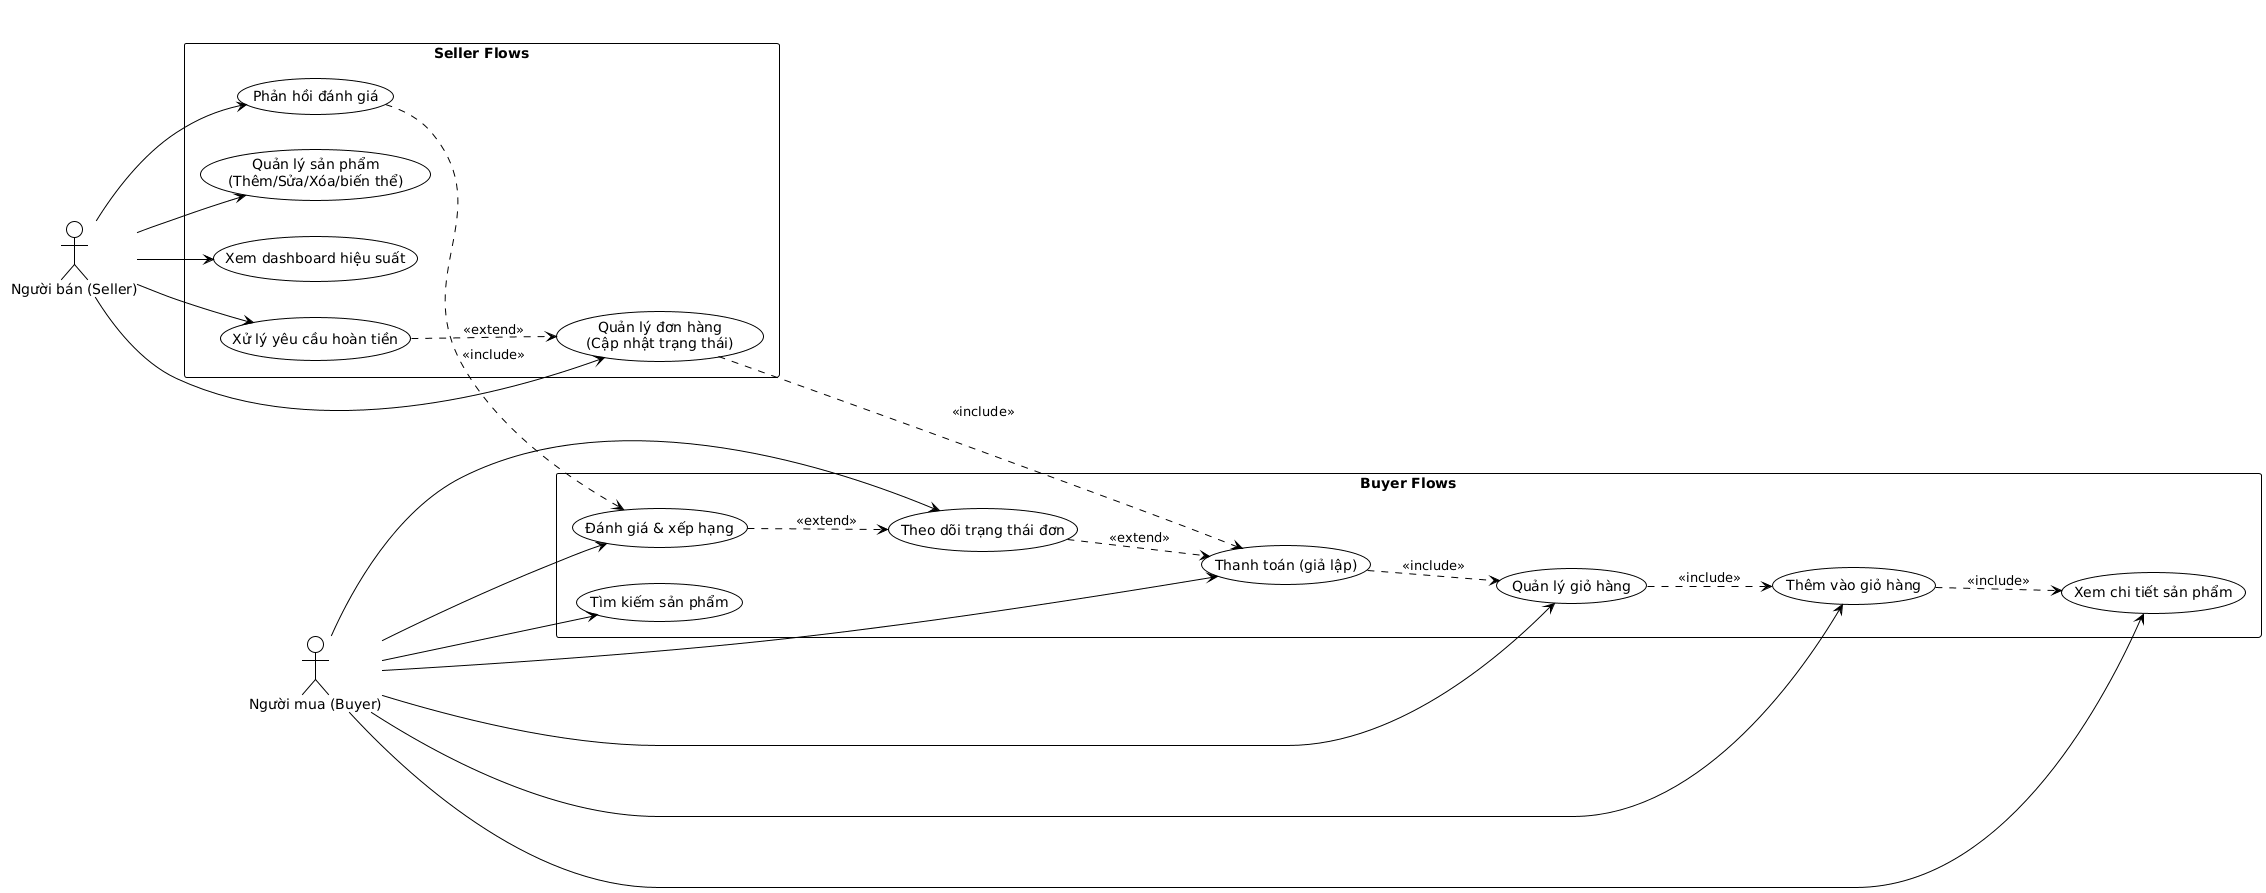
\includegraphics[width=\textwidth]{Images/Usecases/UC-M3-Commerce.png}
\caption{Sơ đồ Use Case cho Module 3: Hoạt động Thương mại}
\label{fig:usecase-module3}
\end{figure}

\renewcommand{\arraystretch}{1.3}

% =====================================================
% PHẦN 1: DÀNH CHO NGƯỜI MUA (BUYER)
% =====================================================
\paragraph{A. Các chức năng dành cho Người mua (Buyer)}

% UC3.1: TÌM KIẾM SẢN PHẨM
\begin{table}[H]
\centering
\begin{tabularx}{\textwidth}{|l|X|}
\hline
\textbf{Tên Use Case} & \textbf{UC3.1: Tìm kiếm sản phẩm} \\ \hline
\textbf{Tác nhân} & Người mua (Buyer) \\ \hline
\textbf{Mô tả} & Cho phép người mua tìm kiếm các sản phẩm họ quan tâm bằng cách sử dụng thanh tìm kiếm và các bộ lọc chi tiết như danh mục và thẻ (tags). \\ \hline
\textbf{Kích hoạt} & Người mua nhập từ khóa vào thanh tìm kiếm hoặc chọn các bộ lọc trên trang sản phẩm. \\ \hline
\textbf{Điều kiện tiên quyết} & Người mua có thể đã đăng nhập hoặc chưa. \\ \hline
\textbf{Điều kiện sau} & Một danh sách các sản phẩm phù hợp với tiêu chí tìm kiếm được hiển thị cho người mua. \\ \hline
\textbf{Luồng sự kiện chính} & 
\begin{enumerate}
    \item Người mua truy cập trang khám phá sản phẩm.
    \item Người mua nhập từ khóa vào thanh tìm kiếm.
    \item Người mua tùy chọn áp dụng các bộ lọc.
    \item Hệ thống truy vấn cơ sở dữ liệu và trả về danh sách sản phẩm khớp.
    \item Giao diện hiển thị kết quả tìm kiếm cho người mua.
\end{enumerate} \\ \hline
\textbf{Ngoại lệ} & E1: Không tìm thấy sản phẩm nào $\rightarrow$ Hệ thống hiển thị thông báo ``Không tìm thấy kết quả phù hợp''. \\ \hline
\end{tabularx}
\caption{Đặc tả Use Case Tìm kiếm sản phẩm}
\end{table}

% UC3.2: XEM CHI TIẾT SẢN PHẨM
\begin{table}[H]
\centering
\begin{tabularx}{\textwidth}{|l|X|}
\hline
\textbf{Tên Use Case} & \textbf{UC3.2: Xem chi tiết sản phẩm} \\ \hline
\textbf{Tác nhân} & Người mua \\ \hline
\textbf{Mô tả} & Cho phép người mua xem thông tin chi tiết về một sản phẩm, bao gồm hình ảnh, mô tả, giá, các biến thể, thông tin người bán và các đánh giá. \\ \hline
\textbf{Kích hoạt} & Người mua nhấp vào một sản phẩm từ kết quả tìm kiếm, Bảng tin hoặc bất kỳ đâu trên nền tảng. \\ \hline
\textbf{Điều kiện tiên quyết} & Sản phẩm phải tồn tại và đang được bán. \\ \hline
\textbf{Điều kiện sau} & Người mua nắm được đầy đủ thông tin về sản phẩm để ra quyết định mua hàng. \\ \hline
\textbf{Luồng sự kiện chính} & 
\begin{enumerate}
    \item Người mua nhấp vào một sản phẩm.
    \item Hệ thống tải và hiển thị trang chi tiết sản phẩm với đầy đủ thông tin.
    \item Người mua có thể xem các hình ảnh, chọn các biến thể (nếu có) và đọc các đánh giá.
\end{enumerate} \\ \hline
\textbf{Ngoại lệ} & E1: Sản phẩm không còn tồn tại hoặc đã bị ẩn $\rightarrow$ Hệ thống hiển thị trang lỗi ``Sản phẩm không tìm thấy''. \\ \hline
\end{tabularx}
\caption{Đặc tả Use Case Xem chi tiết sản phẩm}
\end{table}

% UC3.3: THÊM VÀO GIỎ HÀNG
\begin{table}[H]
\centering
\begin{tabularx}{\textwidth}{|l|X|}
\hline
\textbf{Tên Use Case} & \textbf{UC3.3: Thêm sản phẩm vào giỏ hàng} \\ \hline
\textbf{Tác nhân} & Người mua \\ \hline
\textbf{Mô tả} & Cho phép người mua thêm sản phẩm, bao gồm các biến thể đã chọn, vào giỏ hàng của mình. Người mua có thể thêm sản phẩm từ nhiều cửa hàng khác nhau. \\ \hline
\textbf{Điều kiện tiên quyết} & 
\begin{itemize}
    \item Người mua đã đăng nhập vào hệ thống.
    \item Người mua đã chọn đầy đủ các biến thể bắt buộc của sản phẩm (nếu có).
\end{itemize} \\ \hline
\textbf{Điều kiện sau} & 
\begin{itemize}
    \item Sản phẩm được thêm vào giỏ hàng của người mua.
    \item Biểu tượng giỏ hàng trên giao diện được cập nhật số lượng.
\end{itemize} \\ \hline
\textbf{Luồng sự kiện chính} & 
\begin{enumerate}
    \item Trên trang chi tiết sản phẩm, người mua chọn số lượng và các biến thể mong muốn.
    \item Người mua nhấn ``Thêm vào giỏ hàng''.
    \item Hệ thống xác định biến thể theo \textit{variantId} (hoặc map từ lựa chọn biến thể), kiểm tra trạng thái sản phẩm và tồn kho.
    \item Hệ thống thêm mới hoặc cập nhật cart item tương ứng trong giỏ hàng của người mua.
    \item Hệ thống hiển thị thông báo thành công.
\end{enumerate} \\ \hline
\textbf{Ngoại lệ} & E1: Sản phẩm đã hết hàng $\rightarrow$ Hệ thống báo lỗi và không cho phép thêm vào giỏ. \\ \hline
\end{tabularx}
\caption{Đặc tả Use Case Thêm vào giỏ hàng}
\end{table}

% UC3.4: QUẢN LÝ GIỎ HÀNG
\begin{table}[H]
\centering
\begin{tabularx}{\textwidth}{|l|X|}
\hline
\textbf{Tên Use Case} & \textbf{UC3.4: Quản lý giỏ hàng} \\ \hline
\textbf{Tác nhân} & Người mua \\ \hline
\textbf{Mô tả} & Cho phép người mua xem lại tất cả sản phẩm trong giỏ hàng, cập nhật số lượng, hoặc xóa sản phẩm khỏi giỏ hàng trước khi thanh toán. \\ \hline
\textbf{Kích hoạt} & Người mua nhấp vào biểu tượng giỏ hàng. \\ \hline
\textbf{Điều kiện tiên quyết} & Người mua đã đăng nhập và có ít nhất một sản phẩm trong giỏ hàng. \\ \hline
\textbf{Điều kiện sau} & Giỏ hàng của người mua được cập nhật theo các thay đổi (số lượng, sản phẩm bị xóa). \\ \hline
\textbf{Luồng sự kiện chính} & 
\begin{enumerate}
    \item Người mua truy cập trang giỏ hàng.
    \item Hệ thống hiển thị danh sách các sản phẩm đã thêm.
    \item Người mua có thể: Tăng/giảm số lượng hoặc xóa sản phẩm.
    \item Hệ thống tự động cập nhật lại tổng số tiền.
\end{enumerate} \\ \hline
\textbf{Ngoại lệ} & E1: Cập nhật số lượng vượt quá số lượng tồn kho $\rightarrow$ Hệ thống báo lỗi. \\ \hline
\end{tabularx}
\caption{Đặc tả Use Case Quản lý giỏ hàng}
\end{table}

% UC3.5: THANH TOÁN
\begin{table}[H]
\centering
\begin{tabularx}{\textwidth}{|l|X|}
\hline
\textbf{Tên Use Case} & \textbf{UC3.5: Thực hiện thanh toán} \\ \hline
\textbf{Tác nhân} & Người mua \\ \hline
\textbf{Mô tả} & Cho phép người mua hoàn tất quy trình mua sắm bằng cách cung cấp thông tin giao hàng và thực hiện thanh toán qua một giao diện giả lập. \\ \hline
\textbf{Điều kiện tiên quyết} & 
\begin{itemize}
    \item Người mua đã đăng nhập.
    \item Giỏ hàng có ít nhất một sản phẩm.
\end{itemize} \\ \hline
\textbf{Điều kiện sau} & 
\begin{itemize}
    \item Một đơn hàng mới được tạo trong hệ thống với trạng thái ``PENDING'' và ``paymentStatus=PENDING''.
    \item Giỏ hàng của người mua được làm rỗng.
    \item Người mua được chuyển đến trang xác nhận đơn hàng thành công.
\end{itemize} \\ \hline
\textbf{Luồng sự kiện chính} & 
\begin{enumerate}
    \item Từ giỏ hàng, người mua nhấn ``Thanh toán''.
    \item Hệ thống kiểm tra tồn kho lần cuối cho từng cart item.
    \item Người mua điền thông tin giao hàng.
    \item Người mua chọn phương thức thanh toán (giả lập).
    \item Người mua xác nhận đơn hàng.
    \item Hệ thống tạo bản ghi Order/OrderItem, chốt đơn giá tại thời điểm đặt hàng và trừ tồn kho.
    \item Hệ thống hiển thị thông báo đặt hàng thành công.
\end{enumerate} \\ \hline
\textbf{Ngoại lệ} & E1: Một sản phẩm trong giỏ đã hết hàng $\rightarrow$ Hệ thống báo lỗi và yêu cầu cập nhật giỏ hàng. \\ \hline
\end{tabularx}
\caption{Đặc tả Use Case Thanh toán}
\end{table}

% UC3.6: THEO DÕI ĐƠN HÀNG
\begin{table}[H]
\centering
\begin{tabularx}{\textwidth}{|l|X|}
\hline
\textbf{Tên Use Case} & \textbf{UC3.6: Theo dõi trạng thái đơn hàng} \\ \hline
\textbf{Tác nhân} & Người mua \\ \hline
\textbf{Mô tả} & Cho phép người mua xem danh sách các đơn hàng đã đặt và theo dõi trạng thái hiện tại của chúng (ví dụ: Đang xử lý, Đang giao, Đã giao). \\ \hline
\textbf{Kích hoạt} & Người mua truy cập vào mục ``Đơn hàng của tôi'' trong trang cá nhân. \\ \hline
\textbf{Điều kiện tiên quyết} & Người mua đã đăng nhập và đã đặt ít nhất một đơn hàng. \\ \hline
\textbf{Điều kiện sau} & Người mua biết được tình trạng hiện tại của đơn hàng. \\ \hline
\textbf{Luồng sự kiện chính} & 
\begin{enumerate}
    \item Người mua vào trang quản lý đơn hàng.
    \item Hệ thống hiển thị danh sách tất cả các đơn hàng đã đặt, kèm theo mã đơn hàng, ngày đặt và trạng thái.
    \item Người mua có thể nhấp vào một đơn hàng để xem chi tiết.
\end{enumerate} \\ \hline
\textbf{Ghi chú} & Trạng thái đơn hàng sẽ do Người bán cập nhật (tham chiếu UC3.10). \\ \hline
\end{tabularx}
\caption{Đặc tả Use Case Theo dõi đơn hàng}
\end{table}

% UC3.7: ĐÁNH GIÁ SẢN PHẨM
\begin{table}[H]
\centering
\begin{tabularx}{\textwidth}{|l|X|}
\hline
\textbf{Tên Use Case} & \textbf{UC3.7: Đánh giá và xếp hạng} \\ \hline
\textbf{Tác nhân} & Người mua \\ \hline
\textbf{Mô tả} & Sau khi mua hàng, người mua có thể để lại phản hồi bằng cách viết đánh giá và cho điểm (xếp hạng sao) cho sản phẩm và người bán. \\ \hline
\textbf{Điều kiện tiên quyết} & 
\begin{itemize}
    \item Người mua đã đăng nhập.
    \item Đơn hàng chứa sản phẩm đó phải ở trạng thái ``Đã giao'' hoặc ``Hoàn thành''.
\end{itemize} \\ \hline
\textbf{Điều kiện sau} & 
\begin{itemize}
    \item Một đánh giá mới được lưu vào cơ sở dữ liệu.
    \item Đánh giá và xếp hạng được hiển thị công khai.
\end{itemize} \\ \hline
\textbf{Luồng sự kiện chính} & 
\begin{enumerate}
    \item Người mua vào mục đơn hàng đã giao hoặc hoàn thành.
    \item Người mua chọn sản phẩm muốn đánh giá và nhấn ``Đánh giá''.
    \item Hệ thống hiển thị form đánh giá (chọn sao, viết bình luận, tải ảnh).
    \item Người mua điền thông tin và nhấn ``Gửi đánh giá''.
    \item Hệ thống xác thực quyền theo \textit{orderItemId} và lưu đánh giá.
\end{enumerate} \\ \hline
\textbf{Ngoại lệ} & E1: Người mua cố gắng đánh giá một sản phẩm họ chưa mua hoặc đã đánh giá trước đó $\rightarrow$ Hệ thống không cho phép. \\ \hline
\textbf{Ghi chú} & Đánh giá là một phần quan trọng để xây dựng lòng tin trong cộng đồng. \\ \hline
\end{tabularx}
\caption{Đặc tả Use Case Đánh giá sản phẩm}
\end{table}

\vspace{1cm}

% =====================================================
% PHẦN 2: DÀNH CHO NGƯỜI BÁN (SELLER)
% =====================================================
\paragraph{B. Các chức năng dành cho Người bán (Seller)}

% UC3.8: QUẢN LÝ SẢN PHẨM
\begin{table}[H]
\centering
\begin{tabularx}{\textwidth}{|l|X|}
\hline
\textbf{Tên Use Case} & \textbf{UC3.8: Quản lý sản phẩm} \\ \hline
\textbf{Tác nhân} & Người bán (Seller) \\ \hline
\textbf{Mô tả} & Cung cấp công cụ để người bán thêm, sửa, xóa sản phẩm và quản lý thông tin nâng cao như biến thể (kích cỡ, màu sắc), danh mục và thẻ. \\ \hline
\textbf{Kích hoạt} & Người bán truy cập vào mục ``Quản lý sản phẩm'' trong Bảng điều khiển của mình. \\ \hline
\textbf{Điều kiện tiên quyết} & Người dùng phải đăng nhập với vai trò Seller. \\ \hline
\textbf{Điều kiện sau} & Danh sách sản phẩm của cửa hàng được cập nhật. \\ \hline
\textbf{Luồng sự kiện chính} & 
\begin{enumerate}
    \item Người bán vào trang quản lý sản phẩm và nhấn ``Thêm sản phẩm mới''.
    \item Người bán điền đầy đủ thông tin: tên, mô tả, giá, tồn kho, hình ảnh...
    \item Người bán tùy chọn thêm các biến thể, danh mục, thẻ.
    \item Người bán nhấn ``Lưu''.
    \item Hệ thống xác thực dữ liệu và tạo một bản ghi sản phẩm mới.
    \item Người bán có thể chọn một sản phẩm có sẵn để ``Sửa'' hoặc ``Xóa''.
\end{enumerate} \\ \hline
\textbf{Ngoại lệ} & E1: Dữ liệu nhập vào không hợp lệ (ví dụ: giá âm) $\rightarrow$ Hệ thống báo lỗi. \\ \hline
\textbf{Ghi chú} & Đây là chức năng cốt lõi cho phép người bán đưa hàng hóa lên nền tảng. \\ \hline
\end{tabularx}
\caption{Đặc tả Use Case Quản lý sản phẩm}
\end{table}

% UC3.9: DASHBOARD
\begin{table}[H]
\centering
\begin{tabularx}{\textwidth}{|l|X|}
\hline
\textbf{Tên Use Case} & \textbf{UC3.9: Xem dashboard hiệu suất} \\ \hline
\textbf{Tác nhân} & Người bán \\ \hline
\textbf{Mô tả} & Cung cấp một Bảng điều khiển (dashboard) trực quan để người bán theo dõi hiệu suất kinh doanh qua các chỉ số như lượt xem, doanh số, số đơn hàng... \\ \hline
\textbf{Kích hoạt} & Người bán truy cập vào trang Dashboard chính sau khi đăng nhập. \\ \hline
\textbf{Điều kiện tiên quyết} & Người dùng phải đăng nhập với vai trò Seller. \\ \hline
\textbf{Điều kiện sau} & Người bán nắm được tình hình kinh doanh tổng quan của mình. \\ \hline
\textbf{Luồng sự kiện chính} & 
\begin{enumerate}
    \item Người bán truy cập trang Dashboard.
    \item Hệ thống tổng hợp dữ liệu trong một khoảng thời gian nhất định.
    \item Hệ thống hiển thị dữ liệu dưới dạng các con số, biểu đồ để dễ theo dõi.
    \item Người bán có thể thay đổi khoảng thời gian xem báo cáo.
\end{enumerate} \\ \hline
\textbf{Ghi chú} & Giúp người bán đưa ra các quyết định kinh doanh tốt hơn. \\ \hline
\end{tabularx}
\caption{Đặc tả Use Case Xem Dashboard}
\end{table}

% UC3.10: QUẢN LÝ ĐƠN HÀNG
\begin{table}[H]
\centering
\begin{tabularx}{\textwidth}{|l|X|}
\hline
\textbf{Tên Use Case} & \textbf{UC3.10: Quản lý đơn hàng} \\ \hline
\textbf{Tác nhân} & Người bán \\ \hline
\textbf{Mô tả} & Cho phép người bán xem danh sách các đơn hàng và cập nhật trạng thái của chúng (ví dụ: từ ``Đang xử lý'' sang ``Đang giao''). \\ \hline
\textbf{Kích hoạt} & Người bán truy cập vào mục ``Quản lý đơn hàng'' trong dashboard. \\ \hline
\textbf{Điều kiện tiên quyết} & 
\begin{itemize}
    \item Người dùng phải đăng nhập với vai trò Seller.
    \item Cửa hàng có ít nhất một đơn hàng.
\end{itemize} \\ \hline
\textbf{Điều kiện sau} & Trạng thái của đơn hàng được cập nhật và người mua sẽ thấy được sự thay đổi này. \\ \hline
\textbf{Luồng sự kiện chính} & 
\begin{enumerate}
    \item Người bán vào trang quản lý đơn hàng.
    \item Hệ thống hiển thị danh sách các đơn hàng mới.
    \item Người bán nhấp vào một đơn hàng để xem chi tiết.
    \item Sau khi chuẩn bị xong, người bán thay đổi trạng thái đơn hàng.
    \item Hệ thống lưu lại trạng thái mới.
\end{enumerate} \\ \hline
\end{tabularx}
\caption{Đặc tả Use Case Quản lý đơn hàng của Shop}
\end{table}

% UC3.11: XỬ LÝ HOÀN TIỀN
\begin{table}[H]
\centering
\begin{tabularx}{\textwidth}{|l|X|}
\hline
\textbf{Tên Use Case} & \textbf{UC3.11: Xử lý yêu cầu hoàn tiền} \\ \hline
\textbf{Tác nhân} & Người bán \\ \hline
\textbf{Mô tả} & Cung cấp một quy trình (giả lập) để người bán xem xét và xử lý các yêu cầu hoàn tiền từ người mua. \\ \hline
\textbf{Kích hoạt} & Một người mua gửi yêu cầu hoàn tiền cho một đơn hàng. \\ \hline
\textbf{Điều kiện tiên quyết} & Người dùng phải đăng nhập với vai trò Seller. \\ \hline
\textbf{Điều kiện sau} & Yêu cầu hoàn tiền được giải quyết (chấp nhận hoặc từ chối). \\ \hline
\textbf{Luồng sự kiện chính} & 
\begin{enumerate}
    \item Người bán nhận được thông báo về một yêu cầu hoàn tiền mới.
    \item Người bán vào mục ``Yêu cầu hoàn tiền'' để xem danh sách yêu cầu có trạng thái chờ xử lý.
    \item Người bán đưa ra quyết định ``Chấp nhận'' hoặc ``Từ chối'' yêu cầu.
    \item Nếu chấp nhận, hệ thống cập nhật đơn hàng sang ``REFUNDED''; nếu từ chối, hệ thống lưu lý do từ chối.
    \item Hệ thống ghi nhận quyết định và thông báo lại cho người mua.
    \item Người bán có thể liên hệ với người mua qua tin nhắn để thảo luận thêm.
\end{enumerate} \\ \hline
\textbf{Ghi chú} & Quy trình này được giả lập trong phạm vi đồ án. \\ \hline
\end{tabularx}
\caption{Đặc tả Use Case Xử lý hoàn tiền}
\end{table}

% UC3.12: PHẢN HỒI ĐÁNH GIÁ
\begin{table}[H]
\centering
\begin{tabularx}{\textwidth}{|l|X|}
\hline
\textbf{Tên Use Case} & \textbf{UC3.12: Phản hồi đánh giá} \\ \hline
\textbf{Tác nhân} & Người bán \\ \hline
\textbf{Mô tả} & Cho phép người bán viết phản hồi công khai cho các đánh giá mà người mua đã để lại, giúp tăng cường tương tác và xây dựng niềm tin. \\ \hline
\textbf{Điều kiện tiên quyết} & 
\begin{itemize}
    \item Người dùng phải đăng nhập với vai trò Seller.
    \item Phải có ít nhất một đánh giá từ người mua.
\end{itemize} \\ \hline
\textbf{Điều kiện sau} & Phản hồi của người bán được lưu và hiển thị ngay bên dưới đánh giá của người mua. \\ \hline
\textbf{Luồng sự kiện chính} & 
\begin{enumerate}
    \item Người bán vào mục quản lý đánh giá.
    \item Người bán chọn một đánh giá và nhấn nút ``Phản hồi''.
    \item Người bán nhập nội dung phản hồi và nhấn gửi.
    \item Hệ thống lưu và hiển thị phản hồi đó.
\end{enumerate} \\ \hline
\textbf{Ghi chú} & Đây là một công cụ tốt để thể hiện sự chuyên nghiệp và chăm sóc khách hàng. \\ \hline
\end{tabularx}
\caption{Đặc tả Use Case Phản hồi đánh giá}
\end{table}

\subsection{Module 4: Hệ thống Quản trị}
\subsubsection{Module 4: Hệ thống Quản trị (Admin System)}
Module này cung cấp các công cụ quyền lực cho Quản trị viên (Admin) để giám sát người dùng, kiểm duyệt nội dung và theo dõi sức khỏe của toàn bộ hệ thống.

\begin{figure}[H]
\centering
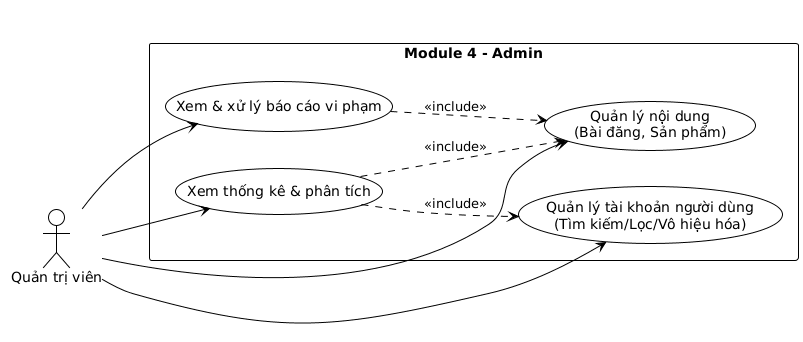
\includegraphics[width=\textwidth]{Images/Usecases/UC-M4-Admin.png}
\caption{Sơ đồ Use Case cho Module 4: Hệ thống Quản trị}
\label{fig:usecase-module4}
\end{figure}

\renewcommand{\arraystretch}{1.3}

% =====================================================
% UC4.1: QUẢN LÝ TÀI KHOẢN NGƯỜI DÙNG
% =====================================================
\begin{table}[H]
\centering
\begin{tabularx}{\textwidth}{|l|X|}
\hline
\textbf{Tên Use Case} & \textbf{UC4.1: Quản lý tài khoản người dùng} \\ \hline
\textbf{Tác nhân} & Quản trị viên (Admin) \\ \hline
\textbf{Mô tả} & Cung cấp cho quản trị viên các công cụ để xem, tìm kiếm, lọc và thực hiện các hành động trên tài khoản người dùng như vô hiệu hóa hoặc cấp lại quyền. \\ \hline
\textbf{Kích hoạt} & Quản trị viên truy cập vào mục ``Quản lý Người dùng'' trong Bảng điều khiển quản trị (Admin Dashboard). \\ \hline
\textbf{Điều kiện tiên quyết} & Quản trị viên đã đăng nhập vào hệ thống với quyền hạn phù hợp. \\ \hline
\textbf{Điều kiện sau} & Thông tin hoặc trạng thái của một hoặc nhiều tài khoản người dùng được thay đổi (ví dụ: tài khoản bị vô hiệu hóa). \\ \hline
\textbf{Luồng sự kiện chính} & 
\begin{enumerate}
    \item Quản trị viên truy cập trang quản lý người dùng.
    \item Hệ thống hiển thị danh sách tất cả người dùng.
    \item Quản trị viên sử dụng các bộ lọc để tìm kiếm người dùng theo tiêu chí.
    \item Quản trị viên chọn một tài khoản người dùng để xem thông tin chi tiết.
    \item Quản trị viên thực hiện một hành động (ví dụ: nhấn nút ``Vô hiệu hóa tài khoản'').
    \item Hệ thống yêu cầu xác nhận hành động.
    \item Quản trị viên xác nhận, và hệ thống cập nhật trạng thái của tài khoản.
\end{enumerate} \\ \hline
\textbf{Ngoại lệ} & 
\begin{itemize}
    \item E1: Quản trị viên cố gắng thực hiện hành động trên tài khoản quản trị viên khác có quyền hạn cao hơn $\rightarrow$ Hệ thống từ chối.
\end{itemize} \\ \hline
\textbf{Ghi chú} & Chức năng này giúp admin duy trì sự kiểm soát đối với cộng đồng người dùng. \\ \hline
\end{tabularx}
\caption{Đặc tả Use Case Quản lý người dùng}
\end{table}

% =====================================================
% UC4.2: QUẢN LÝ NỘI DUNG
% =====================================================
\begin{table}[H]
\centering
\begin{tabularx}{\textwidth}{|l|X|}
\hline
\textbf{Tên Use Case} & \textbf{UC4.2: Quản lý nội dung (Bài đăng/Sản phẩm)} \\ \hline
\textbf{Tác nhân} & Quản trị viên \\ \hline
\textbf{Mô tả} & Cho phép quản trị viên tìm kiếm, xem và xóa các nội dung do người dùng tạo ra như bài đăng hoặc sản phẩm không phù hợp. \\ \hline
\textbf{Kích hoạt} & Quản trị viên truy cập vào các mục quản lý nội dung (ví dụ: ``Quản lý Bài đăng'', ``Quản lý Sản phẩm'') trong dashboard. \\ \hline
\textbf{Điều kiện tiên quyết} & Quản trị viên đã đăng nhập vào hệ thống. \\ \hline
\textbf{Điều kiện sau} & Nội dung không phù hợp (bài đăng, sản phẩm) bị xóa khỏi hệ thống. \\ \hline
\textbf{Luồng sự kiện chính} & 
\begin{enumerate}
    \item Quản trị viên chọn mục nội dung cần quản lý.
    \item Hệ thống hiển thị danh sách các nội dung liên quan.
    \item Quản trị viên sử dụng bộ lọc để tìm kiếm nội dung.
    \item Quản trị viên chọn một nội dung để xem xét.
    \item Nếu nội dung vi phạm, quản trị viên nhấn nút ``Xóa''.
    \item Hệ thống xác nhận và xóa nội dung khỏi cơ sở dữ liệu.
\end{enumerate} \\ \hline
\textbf{Ghi chú} & Việc kiểm duyệt nội dung là cần thiết để giữ cho nền tảng lành mạnh. \\ \hline
\end{tabularx}
\caption{Đặc tả Use Case Quản lý nội dung}
\end{table}

% =====================================================
% UC4.3: XỬ LÝ BÁO CÁO VI PHẠM
% =====================================================
\begin{table}[H]
\centering
\begin{tabularx}{\textwidth}{|l|X|}
\hline
\textbf{Tên Use Case} & \textbf{UC4.3: Xem và xử lý báo cáo vi phạm} \\ \hline
\textbf{Tác nhân} & Quản trị viên \\ \hline
\textbf{Mô tả} & Cho phép quản trị viên xem lại các báo cáo vi phạm được gửi bởi người dùng và đưa ra hành động xử lý phù hợp (ví dụ: xóa nội dung, khóa tài khoản). \\ \hline
\textbf{Điều kiện tiên quyết} & 
\begin{itemize}
    \item Quản trị viên đã đăng nhập vào hệ thống.
    \item Có ít nhất một báo cáo từ người dùng được gửi đến hệ thống.
\end{itemize} \\ \hline
\textbf{Điều kiện sau} & 
\begin{itemize}
    \item Báo cáo được đánh dấu là ``đã xử lý''.
    \item Hành động xử lý đối với nội dung hoặc người dùng bị báo cáo được thực thi.
\end{itemize} \\ \hline
\textbf{Luồng sự kiện chính} & 
\begin{enumerate}
    \item Quản trị viên vào trang quản lý báo cáo.
    \item Hệ thống hiển thị danh sách các báo cáo chưa được xử lý, sắp xếp theo mức độ ưu tiên.
    \item Quản trị viên chọn một báo cáo để xem chi tiết.
    \item Quản trị viên điều hướng đến nội dung/người dùng bị báo cáo để kiểm tra.
    \item Dựa trên kết quả, quản trị viên quyết định hành động (ví dụ: Xóa bài đăng).
    \item Quản trị viên thực hiện hành động thông qua các công cụ quản lý.
    \item Quản trị viên đánh dấu báo cáo là ``Đã xử lý''.
\end{enumerate} \\ \hline
\textbf{Luồng thay thế} & 
\begin{itemize}
    \item A1: Quản trị viên xác định báo cáo là không hợp lệ và đánh dấu là ``Từ chối''.
\end{itemize} \\ \hline
\textbf{Ngoại lệ} & 
\begin{itemize}
    \item E1: Nội dung bị báo cáo đã được người dùng tự xóa trước khi admin xử lý $\rightarrow$ Admin đánh dấu báo cáo là đã giải quyết.
\end{itemize} \\ \hline
\textbf{Ghi chú} & Đây là chức năng tương tác trực tiếp với phản hồi của cộng đồng để duy trì một môi trường an toàn. \\ \hline
\end{tabularx}
\caption{Đặc tả Use Case Xử lý báo cáo}
\end{table}

% =====================================================
% UC4.4: THỐNG KÊ HỆ THỐNG
% =====================================================
\begin{table}[H]
\centering
\begin{tabularx}{\textwidth}{|l|X|}
\hline
\textbf{Tên Use Case} & \textbf{UC4.4: Xem thống kê và phân tích hệ thống} \\ \hline
\textbf{Tác nhân} & Quản trị viên \\ \hline
\textbf{Mô tả} & Cung cấp các biểu đồ và số liệu thống kê trực quan để quản trị viên theo dõi sự phát triển và ``sức khỏe'' của nền tảng. \\ \hline
\textbf{Kích hoạt} & Quản trị viên truy cập vào mục ``Thống kê \& Phân tích'' trong dashboard. \\ \hline
\textbf{Điều kiện tiên quyết} & Quản trị viên đã đăng nhập vào hệ thống. \\ \hline
\textbf{Điều kiện sau} & Quản trị viên nắm được các chỉ số quan trọng về hoạt động của hệ thống để đưa ra quyết định vận hành. \\ \hline
\textbf{Luồng sự kiện chính} & 
\begin{enumerate}
    \item Quản trị viên truy cập trang thống kê.
    \item Hệ thống truy vấn và tổng hợp dữ liệu.
    \item Hệ thống hiển thị các thông tin tổng quan (tổng số người dùng, sản phẩm, bài đăng).
    \item Hệ thống hiển thị các biểu đồ trực quan, chẳng hạn như: Biểu đồ đường thể hiện số lượng người dùng mới; Biểu đồ tròn thể hiện tỷ lệ giữa người mua và người bán.
    \item Quản trị viên có thể thay đổi khoảng thời gian xem thống kê (ví dụ: 7 ngày qua, 30 ngày qua).
\end{enumerate} \\ \hline
\textbf{Ngoại lệ} & 
\begin{itemize}
    \item E1: Lỗi khi tổng hợp dữ liệu $\rightarrow$ Hệ thống báo lỗi.
\end{itemize} \\ \hline
\textbf{Ghi chú} & Các công cụ phân tích này rất quan trọng để theo dõi sự tăng trưởng của hệ thống. \\ \hline
\end{tabularx}
\caption{Đặc tả Use Case Thống kê hệ thống}
\end{table}

\subsection{Module 5: Tích hợp AI Hỗ trợ Sáng tạo Nội dung}
\subsubsection{Module 5: Tích hợp AI Hỗ trợ Sáng tạo}
Đây là tính năng điểm nhấn của dự án, sử dụng Google Gemini API để hỗ trợ người dùng và người bán tạo nội dung đa phương thức chất lượng cao một cách tự động, bao gồm văn bản, hình ảnh và video ngắn. Hệ thống áp dụng pipeline \textbf{Evaluate--Refine Loop}: sau khi gọi API tạo nội dung, kết quả được đánh giá tự động theo các tiêu chí chất lượng (thang điểm 1--10, ngưỡng chấp nhận $\geq$ 7.0). Nếu chưa đạt, hệ thống tự động sửa prompt và thử lại (tối đa 3 lần) trước khi trả kết quả tốt nhất kèm gợi ý chỉnh sửa cho người dùng.

\begin{figure}[H]
\centering
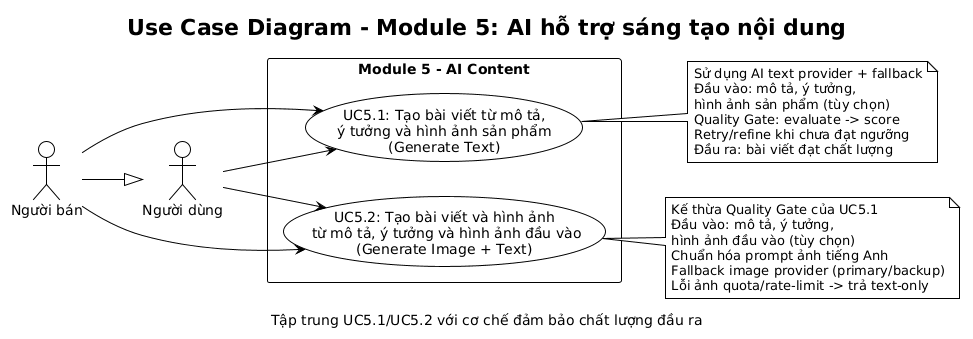
\includegraphics[width=\textwidth]{Images/Usecases/UC-M5-AI.png}
\caption{Sơ đồ Use Case cho Module 5: Tích hợp AI Hỗ trợ Sáng tạo}
\label{fig:usecase-module5}
\end{figure}

\renewcommand{\arraystretch}{1.3}

% UC5.1: GENERATE TEXT
\begin{longtable}{|p{3.5cm}|p{11cm}|}
\caption{Đặc tả Use Case AI Generate Text} \label{tab:uc5.1} \\
\hline
\endfirsthead

\multicolumn{2}{c}%
{{\bfseries \tablename\ \thetable{} -- tiếp tục từ trang trước}} \\
\hline
\endhead

\hline \multicolumn{2}{|r|}{{Tiếp tục ở trang sau}} \\ \hline
\endfoot

\hline
\endlastfoot

\textbf{Tên Use Case} & \textbf{UC5.1: Tạo bài viết từ mô tả, ý tưởng và hình ảnh sản phẩm (Generate Text)} \\ \hline
\textbf{Tác nhân} & Người dùng, Người bán \\ \hline
\textbf{Mô tả} & Cho phép người dùng tạo ra một bài viết hoàn chỉnh dựa trên mô tả, ý tưởng và hình ảnh sản phẩm (nếu có) sử dụng Google Gemini API, với quy trình đánh giá chất lượng tự động và cải thiện prompt khi kết quả chưa đạt. \\ \hline
\textbf{Kích hoạt} & Khi đang soạn thảo bài đăng, người dùng nhấn vào tùy chọn ``Tạo bài viết với AI''. \\ \hline
\textbf{Điều kiện tiên quyết} & 
\begin{itemize}
    \item Người dùng đã đăng nhập và đang trong giao diện tạo bài đăng.
    \item Người dùng đã nhập ít nhất một mô tả hoặc ý tưởng, có thể kèm theo hình ảnh sản phẩm.
\end{itemize} \\ \hline
\textbf{Điều kiện sau} & Một nội dung bài viết hoàn chỉnh (tiêu đề, nội dung, hashtags, CTA) được tạo ra và chèn vào trình soạn thảo, kèm theo điểm đánh giá chất lượng và gợi ý chỉnh sửa (nếu có). \\ \hline
\textbf{Luồng sự kiện chính} & 
\begin{enumerate}
    \item Người dùng nhập mô tả hoặc ý tưởng về bài viết (có thể tải lên hình ảnh sản phẩm).
    \item Người dùng nhấn nút ``Tạo bài viết với AI''.
    \item Hệ thống phân tích đầu vào: trích xuất thực thể chính (tên sản phẩm, đặc điểm, lợi ích), xác định giọng điệu và loại nội dung. Nếu có hình ảnh, phân tích nội dung hình ảnh bằng Gemini Vision.
    \item Hệ thống xây dựng prompt có cấu trúc gồm 5 phần: System Instruction (vai trò chuyên gia nội dung), Context (thông tin thương hiệu, nền tảng), User Input (mô tả + phân tích hình ảnh), Constraints (độ dài 100--300 từ, 5--10 hashtag, phải có CTA), Output Format (JSON schema).
    \item Hệ thống gửi prompt đến Google Gemini API và nhận kết quả.
    \item Hệ thống đánh giá chất lượng kết quả theo 6 tiêu chí có trọng số: Tính liên quan (0.25), Tính hấp dẫn (0.20), Cấu trúc hoàn chỉnh (0.15), Độ dài phù hợp (0.10), Chất lượng ngôn ngữ (0.15), Giá trị thương mại (0.15). Điểm tổng hợp là trung bình có trọng số.
    \item Nếu điểm $\geq$ 7.0/10: hệ thống hiển thị kết quả kèm điểm đánh giá. Nếu điểm $<$ 7.0 và chưa đạt giới hạn 3 lần thử: hệ thống xác định tiêu chí yếu nhất, bổ sung ràng buộc tương ứng vào prompt và gọi lại API (quay lại bước 5). Nếu đã hết lần thử: trả kết quả tốt nhất kèm gợi ý chỉnh sửa.
    \item Hệ thống hiển thị nội dung trong trình soạn thảo kèm điểm đánh giá chi tiết từng tiêu chí và gợi ý cải thiện.
\end{enumerate} \\ \hline
\textbf{Luồng thay thế} & 
\begin{itemize}
    \item A1: Người dùng không hài lòng với kết quả và nhấn ``Tạo lại'' để pipeline chạy lại từ đầu với prompt mới.
    \item A2: Người dùng chỉnh sửa trực tiếp nội dung trong editor (sửa tiêu đề, nội dung, thêm/bớt hashtag).
    \item A3: Người dùng chọn ``Viết lại đoạn này'' để AI viết lại chỉ đoạn được chọn với hướng dẫn cụ thể.
    \item A4: Người dùng thay đổi giọng điệu (chuyên nghiệp, thân thiện, hài hước, sang trọng) và yêu cầu AI viết lại theo giọng điệu mới.
\end{itemize} \\ \hline
\textbf{Ngoại lệ} & 
\begin{itemize}
    \item E1: Lỗi kết nối đến Gemini API $\rightarrow$ Hệ thống báo lỗi ``Không thể tạo nội dung lúc này, vui lòng thử lại sau''.
    \item E2: Hình ảnh không hợp lệ hoặc quá lớn $\rightarrow$ Hệ thống báo lỗi và yêu cầu tải lại hình ảnh.
    \item E3: Gemini API trả về nội dung vi phạm chính sách $\rightarrow$ Hệ thống lọc và yêu cầu tạo lại với prompt đã điều chỉnh.
\end{itemize} \\ \hline
\textbf{Ghi chú} & Pipeline sử dụng chính Gemini API để đánh giá chất lượng (meta-evaluation), kết hợp kiểm tra quy tắc tự động cho các tiêu chí có thể đo lường (format, length, hashtag count). Điểm đánh giá được hiển thị cho người dùng dưới dạng trực quan (thanh tiến trình hoặc biểu đồ radar). \\ \hline
\end{longtable}

% UC5.2: GENERATE IMAGE + TEXT
\begin{longtable}{|p{3.5cm}|p{11cm}|}
\caption{Đặc tả Use Case AI Generate Image + Text} \label{tab:uc5.2} \\
\hline
\endfirsthead

\multicolumn{2}{c}%
{{\bfseries \tablename\ \thetable{} -- tiếp tục từ trang trước}} \\
\hline
\endhead

\hline \multicolumn{2}{|r|}{{Tiếp tục ở trang sau}} \\ \hline
\endfoot

\hline
\endlastfoot

\textbf{Tên Use Case} & \textbf{UC5.2: Tạo bài viết và hình ảnh từ mô tả, ý tưởng và hình ảnh đầu vào (Generate Image + Text)} \\ \hline
\textbf{Tác nhân} & Người dùng, Người bán \\ \hline
\textbf{Mô tả} & Cho phép người dùng tự động tạo ra bài viết kèm hình ảnh dựa trên mô tả, ý tưởng và hình ảnh đầu vào (nếu có) sử dụng Google Gemini API, với đánh giá chất lượng riêng biệt cho text và image. \\ \hline
\textbf{Kích hoạt} & Khi đang soạn thảo bài đăng, người dùng nhấn vào tùy chọn ``Tạo bài viết và hình ảnh với AI''. \\ \hline
\textbf{Điều kiện tiên quyết} & 
\begin{itemize}
    \item Người dùng đã đăng nhập và đang trong giao diện tạo bài đăng.
    \item Người dùng đã nhập ít nhất một mô tả hoặc ý tưởng, có thể kèm theo hình ảnh đầu vào.
\end{itemize} \\ \hline
\textbf{Điều kiện sau} & Một bài viết hoàn chỉnh kèm hình ảnh được tạo bởi AI, cả hai đều được chèn vào trình soạn thảo kèm điểm đánh giá riêng biệt. \\ \hline
\textbf{Luồng sự kiện chính} & 
\begin{enumerate}
    \item Người dùng nhập mô tả hoặc ý tưởng (có thể tải lên hình ảnh đầu vào để tham khảo).
    \item Người dùng nhấn nút ``Tạo bài viết và hình ảnh với AI''.
    \item Hệ thống phân tích đầu vào (tương tự UC5.1), bổ sung phân tích phong cách hình ảnh (màu sắc chủ đạo, bố cục, đối tượng trong ảnh đầu vào).
    \item Hệ thống xây dựng prompt kép: prompt text (5 phần như UC5.1) và prompt image (System Instruction, Context từ text đã tạo, Visual Spec, Constraints về tỷ lệ 1:1/4:5, Negative Prompt).
    \item Hệ thống tạo text trước (với Evaluate--Refine Loop cho text), sau đó sử dụng text đã tạo làm context để tạo image (với Evaluate--Refine Loop riêng cho image).
    \item Đánh giá text: 6 tiêu chí (như UC5.1). Đánh giá image: 4 tiêu chí -- Tính liên quan (0.30), Chất lượng kỹ thuật (0.25), Tính thẩm mỹ (0.25), Nhất quán thương hiệu (0.20). Mỗi loại phải đạt $\geq$ 7.0/10.
    \item Nếu chỉ text hoặc chỉ image chưa đạt: hệ thống chỉ tạo lại phần chưa đạt, giữ nguyên phần đã tốt.
    \item Hệ thống hiển thị bài viết và hình ảnh kèm điểm đánh giá riêng cho từng loại.
\end{enumerate} \\ \hline
\textbf{Luồng thay thế} & 
\begin{itemize}
    \item A1: Người dùng nhấn ``Tạo lại'' để pipeline chạy lại từ đầu.
    \item A2: Người dùng chỉnh sửa text hoặc thay thế hình ảnh riêng biệt.
    \item A3: Người dùng chọn phong cách hình ảnh khác (photorealistic, illustration, flat design) và yêu cầu tạo lại chỉ hình ảnh.
    \item A4: Người dùng tải lên hình ảnh thay thế từ thiết bị, chỉ sử dụng text do AI tạo.
    \item A5: Người dùng yêu cầu AI chỉnh sửa hình ảnh cụ thể (thay đổi màu nền, thêm/bớt đối tượng).
\end{itemize} \\ \hline
\textbf{Ngoại lệ} & 
\begin{itemize}
    \item E1: Lỗi kết nối đến Gemini API $\rightarrow$ Hệ thống báo lỗi ``Không thể tạo nội dung lúc này, vui lòng thử lại sau''.
    \item E2: Gemini API không thể tạo hình ảnh phù hợp sau 3 lần thử $\rightarrow$ Hệ thống trả về bài viết kèm thông báo và gợi ý chỉnh sửa prompt hình ảnh.
    \item E3: Hình ảnh đầu vào không hợp lệ $\rightarrow$ Hệ thống báo lỗi và yêu cầu tải lại hình ảnh.
\end{itemize} \\ \hline
\textbf{Ghi chú} & Hai Evaluate--Refine Loop chạy tuần tự (text trước, image sau) để đảm bảo hình ảnh phù hợp với nội dung text. Chỉ phần chưa đạt ngưỡng mới được tạo lại, tối ưu chi phí gọi API. \\ \hline
\end{longtable}

% UC5.3: GENERATE VIDEO + IMAGES + TEXT
\begin{longtable}{|p{3.5cm}|p{11cm}|}
\caption{Đặc tả Use Case AI Generate Video + Images + Text} \label{tab:uc5.3} \\
\hline
\endfirsthead

\multicolumn{2}{c}%
{{\bfseries \tablename\ \thetable{} -- tiếp tục từ trang trước}} \\
\hline
\endhead

\hline \multicolumn{2}{|r|}{{Tiếp tục ở trang sau}} \\ \hline
\endfoot

\hline
\endlastfoot

\textbf{Tên Use Case} & \textbf{UC5.3: Tạo video ngắn, hình ảnh và bài viết từ mô tả, ý tưởng và hình ảnh đầu vào (Generate Video + Images + Text)} \\ \hline
\textbf{Tác nhân} & Người dùng, Người bán \\ \hline
\textbf{Mô tả} & Tính năng AI nâng cao nhất, tạo bài đăng đa phương thức (video ngắn + tối đa 3 hình ảnh + bài viết) với pipeline đánh giá ba tầng độc lập, sử dụng Google Gemini API và Google Veo 2. \\ \hline
\textbf{Kích hoạt} & Khi đang soạn thảo bài đăng, người dùng nhấn vào tùy chọn ``Tạo video và nội dung đa phương thức với AI''. \\ \hline
\textbf{Điều kiện tiên quyết} & 
\begin{itemize}
    \item Người dùng đã đăng nhập và đang trong giao diện tạo bài đăng.
    \item Người dùng đã nhập ít nhất một mô tả hoặc ý tưởng, có thể kèm theo hình ảnh đầu vào.
\end{itemize} \\ \hline
\textbf{Điều kiện sau} & Một bài đăng đa phương thức hoàn chỉnh (video + images + text) kèm điểm đánh giá từng loại được chèn vào trình soạn thảo. \\ \hline
\textbf{Luồng sự kiện chính} & 
\begin{enumerate}
    \item Người dùng nhập mô tả hoặc ý tưởng (có thể tải lên hình ảnh đầu vào).
    \item Người dùng nhấn nút ``Tạo video và nội dung đa phương thức với AI''.
    \item Hệ thống phân tích đầu vào (tương tự UC5.2), bổ sung xác định storyboard concept (cảnh mở đầu, giới thiệu, highlight, CTA).
    \item Hệ thống thực hiện pipeline tuần tự ba tầng:
    \begin{itemize}
        \item \textbf{Tầng 1 -- Text}: Xây dựng prompt text $\rightarrow$ Gemini API $\rightarrow$ Đánh giá 6 tiêu chí $\rightarrow$ Evaluate--Refine Loop (tối đa 3 lần).
        \item \textbf{Tầng 2 -- Images}: Dùng text làm context $\rightarrow$ Xây dựng prompt image $\rightarrow$ Gemini API tạo tối đa 3 ảnh $\rightarrow$ Đánh giá 4 tiêu chí mỗi ảnh $\rightarrow$ Evaluate--Refine Loop.
        \item \textbf{Tầng 3 -- Video}: Dùng text + images làm context $\rightarrow$ Tự động tạo storyboard $\rightarrow$ Xây dựng prompt video (15--30 giây, tỷ lệ 9:16/1:1) $\rightarrow$ Google Veo 2 $\rightarrow$ Đánh giá 5 tiêu chí: Tính mạch lạc (0.25), Chất lượng hình ảnh (0.25), Độ dài phù hợp (0.15), Tính hấp dẫn (0.20), Nhất quán nội dung (0.15) $\rightarrow$ Evaluate--Refine Loop.
    \end{itemize}
    \item Mỗi tầng Evaluate--Refine Loop chạy độc lập. Khi tạo lại tầng sau, kết quả tầng trước đã đạt được giữ nguyên.
    \item Hệ thống hiển thị video, hình ảnh và bài viết kèm điểm đánh giá chi tiết từng loại. Người dùng có thể chỉnh sửa hoặc tạo lại riêng từng thành phần.
\end{enumerate} \\ \hline
\textbf{Luồng thay thế} & 
\begin{itemize}
    \item A1: Người dùng nhấn ``Tạo lại'' toàn bộ để pipeline chạy lại từ đầu.
    \item A2: Người dùng tạo lại chỉ một thành phần (ví dụ: chỉ video) với yêu cầu bổ sung.
    \item A3: Người dùng chỉnh sửa text, thay thế hình ảnh hoặc video trước khi đăng.
    \item A4: Người dùng cung cấp storyboard chi tiết hơn để cải thiện chất lượng video.
    \item A5: Người dùng chỉ sử dụng một phần nội dung (ví dụ: text + images, bỏ video).
\end{itemize} \\ \hline
\textbf{Ngoại lệ} & 
\begin{itemize}
    \item E1: Lỗi kết nối đến Gemini API hoặc Google Veo 2 $\rightarrow$ Hệ thống báo lỗi.
    \item E2: Gemini API không thể tạo video phù hợp sau 3 lần thử $\rightarrow$ Hệ thống trả về images + text kèm gợi ý cải thiện prompt video.
    \item E3: Hình ảnh đầu vào không hợp lệ $\rightarrow$ Hệ thống báo lỗi.
    \item E4: Video vượt quá 30 giây $\rightarrow$ Kiểm tra rule-based đánh trượt, tự động tạo lại với ràng buộc thời lượng chặt hơn.
\end{itemize} \\ \hline
\textbf{Ghi chú} & Pipeline ba tầng đảm bảo tính nhất quán: text làm nền tảng cho images, text + images làm nền tảng cho video. Đánh giá ``Nhất quán nội dung'' (tiêu chí video) kiểm tra phong cách video có khớp với images và text đã tạo. \\ \hline
\end{longtable}

\subsection{Module 6: Lên lịch và Điều phối Bài đăng}
\subsubsection{Module 6: Lên lịch và Điều phối}
Module này cung cấp tiện ích giúp người dùng và người bán quản lý thời gian đăng bài hiệu quả, đảm bảo nội dung tiếp cận người xem vào khung giờ vàng.

\begin{figure}[H]
\centering
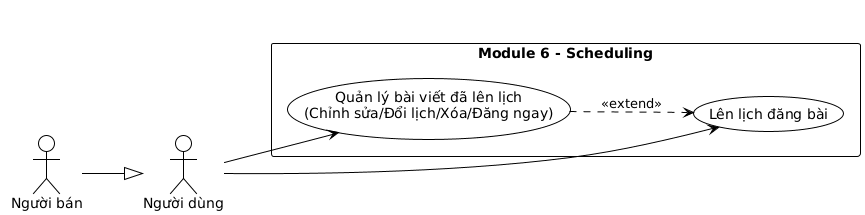
\includegraphics[width=\textwidth]{Images/Usecases/UC-M6-Scheduling.png}
\caption{Sơ đồ Use Case cho Module 6: Lên lịch và Điều phối Bài đăng}
\label{fig:usecase-module6}
\end{figure}

\renewcommand{\arraystretch}{1.3}

% UC6.1: LÊN LỊCH
\begin{table}[H]
\centering
\begin{tabularx}{\textwidth}{|l|X|}
\hline
\textbf{Tên Use Case} & \textbf{UC6.1: Lên lịch đăng bài} \\ \hline
\textbf{Tác nhân} & Người dùng, Người bán \\ \hline
\textbf{Mô tả} & Cung cấp cho người dùng tùy chọn để lên lịch cho một bài đăng, giúp bài viết được tự động xuất bản vào một thời điểm cụ thể trong tương lai. \\ \hline
\textbf{Kích hoạt} & Khi tạo một bài đăng mới, người dùng chọn tùy chọn ``Lên lịch'' thay vì ``Đăng ngay''. \\ \hline
\textbf{Điều kiện tiên quyết} & 
\begin{itemize}
    \item Người dùng đã đăng nhập vào hệ thống.
    \item Người dùng đang ở trong giao diện tạo bài đăng và đã có nội dung cho bài viết.
\end{itemize} \\ \hline
\textbf{Điều kiện sau} & 
\begin{itemize}
    \item Bài đăng được lưu vào cơ sở dữ liệu dưới dạng ``bản nháp đã lên lịch''.
    \item Bài đăng sẽ không hiển thị công khai cho đến đúng thời điểm đã được lên lịch.
\end{itemize} \\ \hline
\textbf{Luồng sự kiện chính} & 
\begin{enumerate}
    \item Trong giao diện tạo bài đăng, sau khi soạn xong nội dung, người dùng chọn tùy chọn ``Lên lịch''.
    \item Một giao diện chọn ngày và giờ trong tương lai sẽ hiện ra.
    \item Người dùng chọn ngày và giờ mong muốn để xuất bản bài viết.
    \item Người dùng nhấn nút ``Xác nhận Lịch''.
    \item Hệ thống lưu bài đăng với trạng thái ``đã lên lịch'' và thời điểm xuất bản đã chọn.
    \item Hệ thống hiển thị thông báo ``Bài viết đã được lên lịch thành công''.
\end{enumerate} \\ \hline
\textbf{Luồng thay thế} & 
\begin{itemize}
    \item A1: Người dùng quyết định không lên lịch nữa và chọn ``Đăng ngay''.
\end{itemize} \\ \hline
\textbf{Ngoại lệ} & 
\begin{itemize}
    \item E1: Người dùng chọn một thời điểm trong quá khứ $\rightarrow$ Hệ thống báo lỗi ``Vui lòng chọn một thời điểm trong tương lai''.
\end{itemize} \\ \hline
\textbf{Ghi chú} & Backend cần có một cơ chế (ví dụ: cron job) để kiểm tra và tự động xuất bản các bài đăng đã đến hạn. \\ \hline
\end{tabularx}
\caption{Đặc tả Use Case Lên lịch đăng bài}
\end{table}

% UC6.2: QUẢN LÝ LỊCH
\begin{table}[H]
\centering
\begin{tabularx}{\textwidth}{|l|X|}
\hline
\textbf{Tên Use Case} & \textbf{UC6.2: Quản lý bài viết đã lên lịch} \\ \hline
\textbf{Tác nhân} & Người dùng, Người bán \\ \hline
\textbf{Mô tả} & Cung cấp một giao diện để người dùng có thể xem lại danh sách các bài viết đang chờ xuất bản, cũng như chỉnh sửa, thay đổi lịch hoặc xóa chúng. \\ \hline
\textbf{Kích hoạt} & Người dùng truy cập vào một mục riêng trong trang cá nhân để xem các bài viết đã lên lịch. \\ \hline
\textbf{Điều kiện tiên quyết} & 
\begin{itemize}
    \item Người dùng đã đăng nhập vào hệ thống.
    \item Người dùng có ít nhất một bài viết đã được lên lịch.
\end{itemize} \\ \hline
\textbf{Điều kiện sau} & Bài viết đã lên lịch được cập nhật (thay đổi nội dung, thời gian) hoặc bị xóa khỏi hàng chờ xuất bản. \\ \hline
\textbf{Luồng sự kiện chính} & 
\begin{enumerate}
    \item Người dùng truy cập vào trang ``Quản lý bài viết đã lên lịch''.
    \item Hệ thống hiển thị danh sách các bài viết đang chờ, kèm theo nội dung xem trước và thời gian dự kiến đăng.
    \item Người dùng chọn một bài viết và thực hiện một trong các hành động: Chỉnh sửa nội dung; Thay đổi lịch; Xóa; Đăng ngay.
    \item Hệ thống cập nhật thay đổi tương ứng vào cơ sở dữ liệu.
\end{enumerate} \\ \hline
\textbf{Luồng thay thế} & 
\begin{itemize}
    \item A1: Người dùng chọn một bài viết và quyết định ``Đăng ngay'' thay vì chờ đến thời gian đã lên lịch.
\end{itemize} \\ \hline
\textbf{Ngoại lệ} & 
\begin{itemize}
    \item E1: Người dùng cố gắng chỉnh sửa một bài viết ngay tại thời điểm nó đang được hệ thống tự động xuất bản $\rightarrow$ Hệ thống báo lỗi hoặc thông báo bài viết đã được đăng.
\end{itemize} \\ \hline
\textbf{Ghi chú} & Giao diện này mang lại sự linh hoạt và quyền kiểm soát hoàn toàn cho người dùng đối với kế hoạch nội dung. \\ \hline
\end{tabularx}
\caption{Đặc tả Use Case Quản lý lịch đăng}
\end{table}

\subsection{Module 7: Hệ thống Thông báo}
\subsubsection{Module 7: Hệ thống Thông báo (Notification)}
Hệ thống thông báo thời gian thực (Real-time) đóng vai trò then chốt trong việc giữ chân người dùng và đảm bảo thông tin mua bán được cập nhật tức thì.

\begin{figure}[H]
\centering
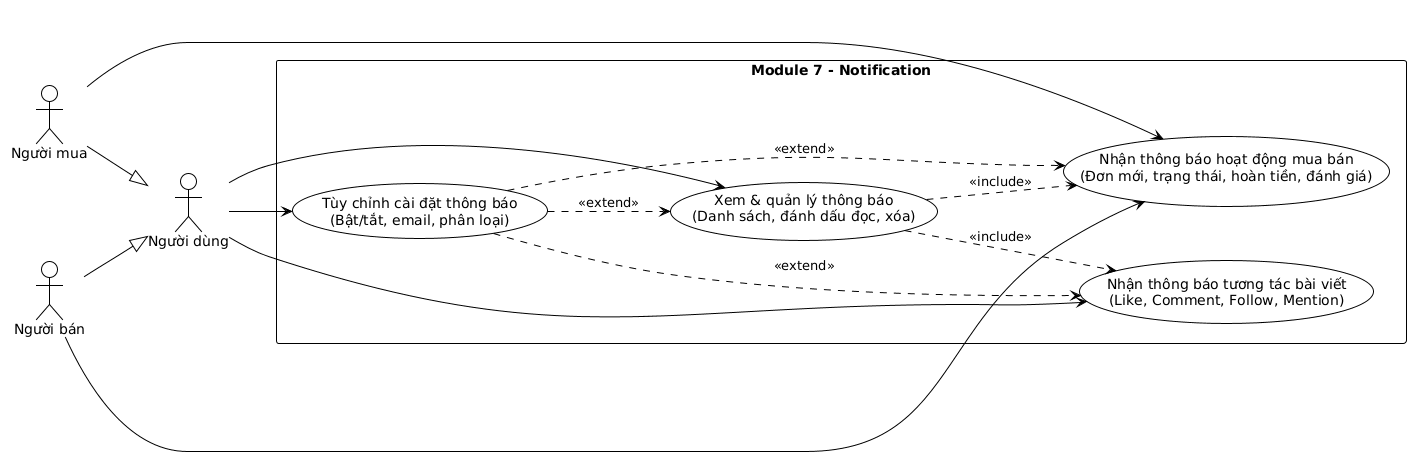
\includegraphics[width=\textwidth]{Images/Usecases/UC-M7-Notification.png}
\caption{Sơ đồ Use Case cho Module 7: Hệ thống Thông báo}
\label{fig:usecase-module7}
\end{figure}

\renewcommand{\arraystretch}{1.3}

% UC7.1: THÔNG BÁO TƯƠNG TÁC
\begin{table}[H]
\centering
\begin{tabularx}{\textwidth}{|l|X|}
\hline
\textbf{Tên Use Case} & \textbf{UC7.1: Nhận thông báo tương tác xã hội} \\ \hline
\textbf{Tác nhân} & Người dùng, Người bán \\ \hline
\textbf{Mô tả} & Hệ thống tự động gửi thông báo ngay lập tức đến người sở hữu bài viết khi có người khác thực hiện các hành động: thích bài viết, bình luận, theo dõi người dùng, hoặc được nhắc đến trong bình luận/bài viết của người khác. \\ \hline
\textbf{Kích hoạt} & Một người dùng khác thực hiện hành động tương tác với bài viết hoặc tài khoản của người nhận. \\ \hline
\textbf{Điều kiện tiên quyết} & 
\begin{itemize}
    \item Người nhận đã đăng nhập vào hệ thống ít nhất một lần trong phiên hiện tại.
    \item Người nhận không tắt hoàn toàn thông báo tương tác xã hội.
\end{itemize} \\ \hline
\textbf{Điều kiện sau} & 
\begin{itemize}
    \item Một thông báo mới xuất hiện trên giao diện người nhận.
    \item Số lượng thông báo chưa đọc tăng lên.
    \item Thông báo được lưu lại để người dùng có thể xem lại sau.
\end{itemize} \\ \hline
\textbf{Luồng sự kiện chính} & 
\begin{enumerate}
    \item Người dùng A thực hiện hành động (ví dụ: thích bài viết của Người dùng B).
    \item Hệ thống phát hiện hành động này.
    \item Hệ thống xác định chủ sở hữu bài viết (Người dùng B).
    \item Hệ thống tạo thông báo mới và gửi ngay lập tức đến Người dùng B.
    \item Giao diện của Người dùng B hiển thị thông báo.
    \item Người dùng B có thể nhấn vào thông báo để chuyển thẳng đến nội dung liên quan.
\end{enumerate} \\ \hline
\textbf{Luồng thay thế} & A1: Người dùng B đang không online $\rightarrow$ Thông báo vẫn được lưu và sẽ hiển thị ngay khi người đó đăng nhập lại. A2: Người dùng B tắt âm thanh thông báo $\rightarrow$ chỉ hiển thị hình ảnh. \\ \hline
\textbf{Ngoại lệ} & 
\begin{itemize}
    \item E1: Người dùng B đã chặn Người dùng A $\rightarrow$ Không gửi thông báo.
    \item E2: Bài viết ở chế độ riêng tư và Người dùng A không được phép xem $\rightarrow$ Không gửi thông báo.
\end{itemize} \\ \hline
\textbf{Ghi chú} & Tính năng quan trọng giúp tăng tính tương tác xã hội. \\ \hline
\end{tabularx}
\caption{Đặc tả Use Case Thông báo tương tác}
\end{table}

% UC7.2: THÔNG BÁO MUA BÁN
\begin{table}[H]
\centering
\begin{tabularx}{\textwidth}{|l|X|}
\hline
\textbf{Tên Use Case} & \textbf{UC7.2: Nhận thông báo hoạt động mua bán} \\ \hline
\textbf{Tác nhân} & Người mua, Người bán \\ \hline
\textbf{Mô tả} & Khi có sự kiện liên quan đến đơn hàng (đặt hàng mới, người bán xác nhận, giao hàng, hoàn thành, hủy đơn, yêu cầu hoàn tiền, có đánh giá mới…), hệ thống gửi thông báo ngay cho cả hai bên liên quan. \\ \hline
\textbf{Kích hoạt} & Bất kỳ thay đổi trạng thái nào của đơn hàng hoặc hành động liên quan đến đơn hàng. \\ \hline
\textbf{Điều kiện tiên quyết} & 
\begin{itemize}
    \item Người nhận có ít nhất một đơn hàng đang trong quá trình xử lý hoặc vừa hoàn tất.
    \item Người nhận chưa tắt thông báo liên quan đến mua bán.
\end{itemize} \\ \hline
\textbf{Điều kiện sau} & 
\begin{itemize}
    \item Cả người mua và người bán đều nhận được thông báo ngay lập tức.
    \item Thông báo chứa liên kết dẫn trực tiếp đến trang chi tiết đơn hàng.
\end{itemize} \\ \hline
\textbf{Luồng sự kiện chính} & 
\begin{enumerate}
    \item Người mua đặt một đơn hàng mới.
    \item Hệ thống tạo thông báo ``Bạn có đơn hàng mới'' gửi đến Người bán.
    \item Người bán xác nhận đơn hàng.
    \item Hệ thống gửi thông báo ``Đơn hàng của bạn đã được xác nhận'' cho Người mua.
    \item Tương tự với các trạng thái: đang giao, đã giao, hoàn thành, hủy, có đánh giá mới, có yêu cầu hoàn tiền…
\end{enumerate} \\ \hline
\textbf{Luồng thay thế} & A1: Một bên đang offline $\rightarrow$ Thông báo được lưu và hiển thị khi đăng nhập lại. A2: Có thể gửi thêm email nếu người dùng bật tùy chọn này. \\ \hline
\textbf{Ngoại lệ} & E1: Đơn hàng bị hủy ngay lập tức bởi người mua trước khi người bán nhìn thấy $\rightarrow$ chỉ gửi thông báo hủy. \\ \hline
\textbf{Ghi chú} & Tính năng này giúp người bán phản hồi nhanh đơn hàng và người mua luôn nắm được trạng thái mua sắm. \\ \hline
\end{tabularx}
\caption{Đặc tả Use Case Thông báo đơn hàng}
\end{table}

% UC7.3: QUẢN LÝ THÔNG BÁO
\begin{table}[H]
\centering
\begin{tabularx}{\textwidth}{|l|X|}
\hline
\textbf{Tên Use Case} & \textbf{UC7.3: Xem và quản lý danh sách thông báo} \\ \hline
\textbf{Tác nhân} & Người dùng \\ \hline
\textbf{Mô tả} & Người dùng có thể mở ra xem toàn bộ danh sách thông báo đã nhận (cả đã đọc và chưa đọc), đánh dấu đã đọc, hoặc xóa thông báo không còn cần thiết. \\ \hline
\textbf{Kích hoạt} & Người dùng nhấn vào biểu tượng chuông hoặc mục ``Thông báo'' trên thanh điều hướng. \\ \hline
\textbf{Điều kiện tiên quyết} & Người dùng đã đăng nhập và từng nhận ít nhất một thông báo. \\ \hline
\textbf{Điều kiện sau} & 
\begin{itemize}
    \item Danh sách thông báo được cập nhật trạng thái đọc/xóa theo hành động của người dùng.
    \item Số lượng thông báo chưa đọc giảm tương ứng.
\end{itemize} \\ \hline
\textbf{Luồng sự kiện chính} & 
\begin{enumerate}
    \item Người dùng nhấn vào biểu tượng thông báo.
    \item Hệ thống hiển thị danh sách tất cả thông báo (mới nhất ở trên).
    \item Thông báo chưa đọc được làm nổi bật.
    \item Người dùng có thể: Nhấn vào thông báo; Đánh dấu đã đọc; Xóa.
    \item Hệ thống cập nhật lại trạng thái và giao diện ngay lập tức.
\end{enumerate} \\ \hline
\textbf{Luồng thay thế} & A1: Người dùng chọn ``Xóa tất cả thông báo'' $\rightarrow$ toàn bộ thông báo bị xóa vĩnh viễn. \\ \hline
\textbf{Ngoại lệ} & E1: Không có thông báo nào $\rightarrow$ hiển thị dòng chữ ``Bạn chưa có thông báo nào''. \\ \hline
\textbf{Ghi chú} & Giao diện nên hỗ trợ phân loại thông báo để dễ theo dõi. \\ \hline
\end{tabularx}
\caption{Đặc tả Use Case Quản lý danh sách thông báo}
\end{table}

% UC7.4: CÀI ĐẶT THÔNG BÁO
\begin{table}[H]
\centering
\begin{tabularx}{\textwidth}{|l|X|}
\hline
\textbf{Tên Use Case} & \textbf{UC7.4: Tùy chỉnh cài đặt thông báo} \\ \hline
\textbf{Tác nhân} & Người dùng \\ \hline
\textbf{Mô tả} & Người dùng có thể tự quyết định sẽ nhận loại thông báo nào, qua kênh nào (trên web, âm thanh, email), và tắt hoàn toàn một số loại thông báo nếu muốn. \\ \hline
\textbf{Kích hoạt} & Người dùng vào phần Cài đặt $\rightarrow$ Thông báo. \\ \hline
\textbf{Điều kiện tiên quyết} & Người dùng đã đăng nhập. \\ \hline
\textbf{Điều kiện sau} & Cài đặt thông báo của người dùng được lưu lại và áp dụng cho mọi phiên đăng nhập sau này. \\ \hline
\textbf{Luồng sự kiện chính} & 
\begin{enumerate}
    \item Người dùng vào Trang cá nhân $\rightarrow$ Cài đặt $\rightarrow$ Thông báo.
    \item Hệ thống hiển thị danh sách các loại thông báo có thể bật/tắt.
    \item Người dùng bật/tắt từng mục và chọn có nhận qua email hay không.
    \item Người dùng nhấn ``Lưu cài đặt''.
    \item Hệ thống lưu và áp dụng ngay lập tức.
\end{enumerate} \\ \hline
\textbf{Luồng thay thế} & A1: Người dùng chọn ``Tắt tất cả thông báo'' $\rightarrow$ toàn bộ thông báo (trừ thông báo hệ thống bắt buộc) sẽ không hiển thị nữa. \\ \hline
\textbf{Ngoại lệ} & Không có. \\ \hline
\textbf{Ghi chú} & Tính năng này quan trọng để tránh làm phiền và tăng trải nghiệm cá nhân hóa. \\ \hline
\end{tabularx}
\caption{Đặc tả Use Case Cài đặt thông báo}
\end{table}